\documentclass[12pt]{article}
\usepackage{geometry}
\geometry{left=1in,right=0.75in,top=1in,bottom=1in}

%%%%%%%%%%%%%%%%%%%%%%%%%%%%%%%%%%%%%%%%
% Replace ABCDEF in the next line with your chosen problem
% and replace 1111111 with your Team Control Number
\newcommand{\Problem}{B}
\newcommand{\Team}{223}
%%%%%%%%%%%%%%%%%%%%%%%%%%%%%%%%%%%%%%%%
\usepackage{newtxtext}
\usepackage{hyperref}
\usepackage{amsmath,amssymb,amsthm}
\usepackage{lipsum}
\usepackage{booktabs}
\usepackage{float}
\usepackage{subfigure}
\usepackage[pdftex]{graphicx}
\usepackage{xcolor}
\usepackage{fancyhdr}
\usepackage{url}
\DeclareUnicodeCharacter{0300}{\'{a}}
\lhead{Team \Team}
\rhead{}
\cfoot{}
\newtheorem{theorem}{Theorem}
\newtheorem{corollary}[theorem]{Corollary}
\newtheorem{lemma}[theorem]{Lemma}
\newtheorem{definition}{Definition}
%%%%%%%%%%%%%%%%%%%%%%%%%%%%%%%%
\begin{document}
\graphicspath{{.}}  % Place your graphic files in the same directory as your main document
\DeclareGraphicsExtensions{.pdf, .jpg, .tif, .png}
\thispagestyle{empty}
\vspace*{-16ex}
\centerline{\begin{tabular}{*3{c}}
	\parbox[t]{0.3\linewidth}{\begin{center}\textbf{Problem Chosen}\\ \Large \textcolor{red}{\Problem}\end{center}}
	& \parbox[t]{0.3\linewidth}{\begin{center}\textbf{2024\\ MCM/ICM\\ Summary Sheet}\end{center}}
	& \parbox[t]{0.3\linewidth}{\begin{center}\textbf{Team Control Number}\\ \Large \textcolor{red}{\Team}\end{center}}	\\
	\hline
\end{tabular}}
%%%%%%%%%%% Begin Summary %%%%%%%%%%%
%标题
\begin{center}
	\Huge {Enhancing Taxi Route Planning: A Comprehensive Analysis of ISPL }\\
	\vspace{0.4cm}
	\normalsize\textbf{Summary}
\end{center}
\vspace{0.2cm}

\indent Taxi companies need to consider user preferences reflected in historical path data because the best route during a taxi ride may not necessarily be the shortest route. It is important to take into account both the distance and user preferences in order to determine the optimal route. Assigning weights to paths based on ambiguous user preferences and planning the shortest path under corresponding conditions belongs to a type of an inverse shortest path length problem(ISPL). To address this problem, we introduce edge PageRank to measure road weights and utilize simulated annealing algorithm to find the maximum SIM value.\\
\indent For the first task, we prove by contradiction that the SIM value in example 1 cannot be equal to 1. Additionally, we attempted to assign weights to each edge, \textbf{resulting in a SIM value of 0.75}.\\
\indent For the second task, we first preprocessed the data in Case 1. We placed the data points on a map of Beijing to observe their distribution characteristics and removed duplicate edges and identified edges that did not appear in any of the paths. We then investigated the number of times each edge was traversed in the paths and analyzed the distribution characteristics of the data.Then, we used \textbf{Dijkstra's algorithm} to find the shortest path length for each path. We sorted the paths in ascending order based on their starting and ending points. By processing all paths with the same starting point at once using an array, we significantly reduced the time complexity. Finally, we calculated that \textbf{the SIM value for Case 1 is 0.248971}.\\
\indent For the third task, in our initial model, we used \textbf{road length, road importance (measured by edge PageRank), and straight-line distance} to measure road weights. We calculated the straight-line distance based on the latitude and longitude of the starting and ending points. We calculated \textbf{the maximum SIM value to be 0.273278}. We then conducted further analysis and found that the straight-line distance had little impact on the SIM value. However, we discovered a significant relationship \textbf{between the data point's index and its location}. Therefore, we decided to optimize our model by excluding the straight-line distance, introduceing the edge index into the calculation formula for edge PageRank and adding a constant. Ultimately, we determined \textbf{several parameters, denoted as 26.27088, 0.01172792, and 0.256358}, to calculate the edge weights. It results in \textbf{a maximum SIM value of 0.298223}.\\
\indent For the fourth task,we first compared the optimization rates of the two models in terms of SIM values obtained compared to using length as edge weights. Next, we plotted scatter plots \textbf{comparing the distribution differences between edge weights and edge lengths}, and analyzed the impact of introducing PageRank into the weight calculation.\\
\indent Finally, we conducted \textbf{sensitivity tests} on the resulting model. We selected the parameters \textbf{strides and initial and final temperatures} for testing and found that the model exhibited good stability for different values of these parameters.\\
%关键词
\vspace{0.4cm}
 \textbf{Keywords: }Route Planning\quad Inverse Shortest Path Length \quad Simulated Annealing Algorithm
%%%%%%%%%%% End Summary %%%%%%%%%%%

%%%%%%%%%%%%%%%%%%%%%%%%%%%%%%
\clearpage
\pagestyle{fancy}
% Uncomment the next line to generate a Table of Contents
%\tableofcontents 
\newpage
\setcounter{page}{2}
\rhead{Page \thepage~of~25}
%%%%%%%%%%%%%%%%%%%%%%%%%%%%%%

%目录
\tableofcontents
\newpage

%正文部分
\section{Introduction}
\subsection{Problem Background}
\subsection{Restatement of the Task}
\subsection{Literature Review}
\subsection{Our Work}
\section{Assumptions and Justifications}
\subsection{Assumptions}
we would like to give the following assumptions://
\begin{itemize}
\item first
\item second
\end{itemize}
\subsection{Justifications}

\section{Notations}
\begin{table}[h]
	\begin{center}
		\begin{tabular}{cc}
			\toprule[1.5pt]
			Symbol&Definition\\
			\midrule[1pt]
			\(x_i\)&Evaluation indicator\\
			\({\tilde x_i}\)&Standardized indicators\\
			\({\mu _i}\)&Average value\\
			\(s_i\)&Standard deviation\\
			\({R}\)&Correlation coefficient matrix\\
			\(y_i\)&Principal Components\\
			\(b_i\)&The information contribution of eigenvalue\\
			\(T\)&Composite score\\
			\bottomrule[1.5pt]
		\end{tabular}
	\end{center}
\end{table}
\section{Model}

%%%%%%%%%%%%%%%%%%%%%%%%%%%%%%%%%%%%%%%%%%%%%%%%%%%%%%%%%%%%%%%%%%%%%%%%%%%%%%%%%%%%
\subsection{Designing Weights to Maxmize the SIM in Example 1}
%第一小节,设计对于例1中各例子的权值,使SIM最大

\indent \indent In the first task, we need to address two issues: what is the maximum SIM in Example 1, and what are the edge weights that result in the maximum SIM. Taking into account that Example 1 only considers four paths with two sets of starting and ending points, namely $(1,7)$ and $(1,9)$, \textbf{SIM can only be one of the values 0, 0.25, 0.5, 0.75, or 1}. In the given example, there are already cases where SIM is 0.25 and 0.5. Therefore, we first aim to determine whether SIM can be 1. If it is possible, then we will proceed to explore the edge weights that meet this condition. Otherwise, we consider \textbf{the case where SIM is 0.75}.\\
\indent We use a \textbf{proof by contradiction} to demonstrate that SIM cannot be equal to 1. As shown in Figure 1, it illustrates the various points and partial edges in Example 1. The letters labeled beside some of the edges represent the lengths of those directed edges. \\
\begin{figure}[H]
    \centering
    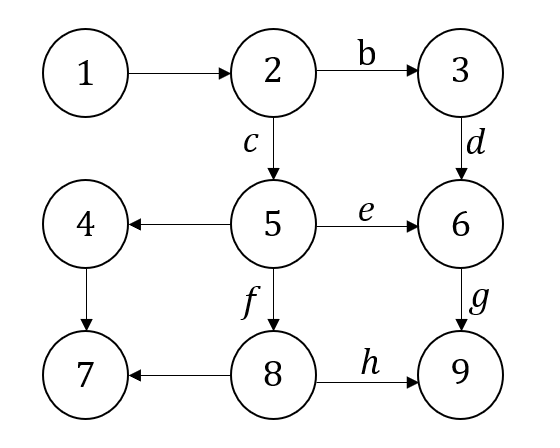
\includegraphics[width=6cm,height=4.5cm]{example1题图.png}
    \caption{Some Edge Weights in Example 1}
\end{figure}
\indent According to the conditions, if the SIM equals to 1, then for paths $p3$ and $p4$, both paths are the shortest path of (1, 9). The relation between the lengths of the two paths is as follows:
\[
\left\{
\begin{aligned}
    c+e+g&=b+d+e+f+h\\
    c+f+h &\geq b+d+e+f+h\\
    b+d+g &\geq c+e+g
\end{aligned}
\right.
\]
\indent We simplify the above equations, and the range of possible values for e can be determined as:
\begin{align*}
    b+d-e \geq c \geq b+d+e 
\end{align*}
\indent To ensure the existence of positive integer solutions for c in the given inequality, we have the following condition for e:
\begin{align*}
    e  \leq  0
\end{align*}
\indent The inequality above \textbf{contradicts the condition stated in the problem that "all path weights are positive integers."} Therefore, the value of the SIM cannot equal to $1$.\\
\indent Since the SIM cannot equal to 1, we begin to seek for cases where the SIM equals to 0.75. We set the weights of the directed edges along paths $p1$, $p2$, and $p3$ to 1, and adjust the weights of the edges $1 \rightarrow 4 $, $2 \rightarrow 3 $, and $8 \rightarrow 9 $ in order to achieve $D(1,7) = D(1,9) = 4$ . Thus, we ensure that $p1$, $p2$, and $p3$ are the shortest paths corresponding to their respective starting and ending points, while $p4$ is not the shortest path. These adjustments result in a SIM value of 0.75. The results are as follows:
\begin{table}[h!]%绘制结果权值表
\begin{center}
    \caption{The Results of the Problem 1}{\vspace{0.5cm}}
    \label{result1}
    \begin{tabular}{|c|c|c|c|c|c|c|c|c|c|c|c|c|c|c|c|c|}
    \hline
    \text{$v_i$}&\text{1}&\text{1}&\text{2}&\text{2}&\text{3}&\text{4}&\text{4}&\text{5}&\text{5}&\text{5}&\text{6}&\text{6}&\text{7}&\text{8}&\text{8}&\text{9}\\
    \hline
    \text{$v_j$}&\text{2}&\text{4}&\text{3}&\text{5}&\text{6}&\text{5}&\text{7}&\text{4}&\text{6}&\text{8}&\text{5}&\text{9}&\text{8}&\text{7}&\text{9}&\text{8}\\
    \hline
    \text{$w$($v_i$,$v_j$)}&\text{1}&\text{4}&\text{4}&\text{1}&\text{1}&\text{1}&\text{1}&\text{1}&\text{1}&\text{1}&\text{1}&\text{1}&\text{1}&\text{1}&\text{4}&\text{1}\\
    \hline
    \end{tabular}
\end{center}
\end{table}

%%%%%%%%%%%%%%%%%%%%%%%%%%%%%%%%%%%%%%%%%%%%%%%%%%%%%%%%%%%%%%%%%%%%%%%%%%%%%%%%%%%%
\subsection{Data Preprocessing for Case 1}
%第二小节:对案例一的数据进行预处理

\indent\indent Due to the large number of data points and edges in Case 1, it is not feasible to obtain the optimal solution through trial and error. Therefore, we need to use a computer program for calculation. Before that, we need to preprocess the data and visualize it in order to better analyze the data based on real-world circumstances.\\
\indent We show all the data points provided in the question on the map of Beijing. The results are as follows:
\begin{figure}[H]%插入图片:初始版北京地图
    \centering
    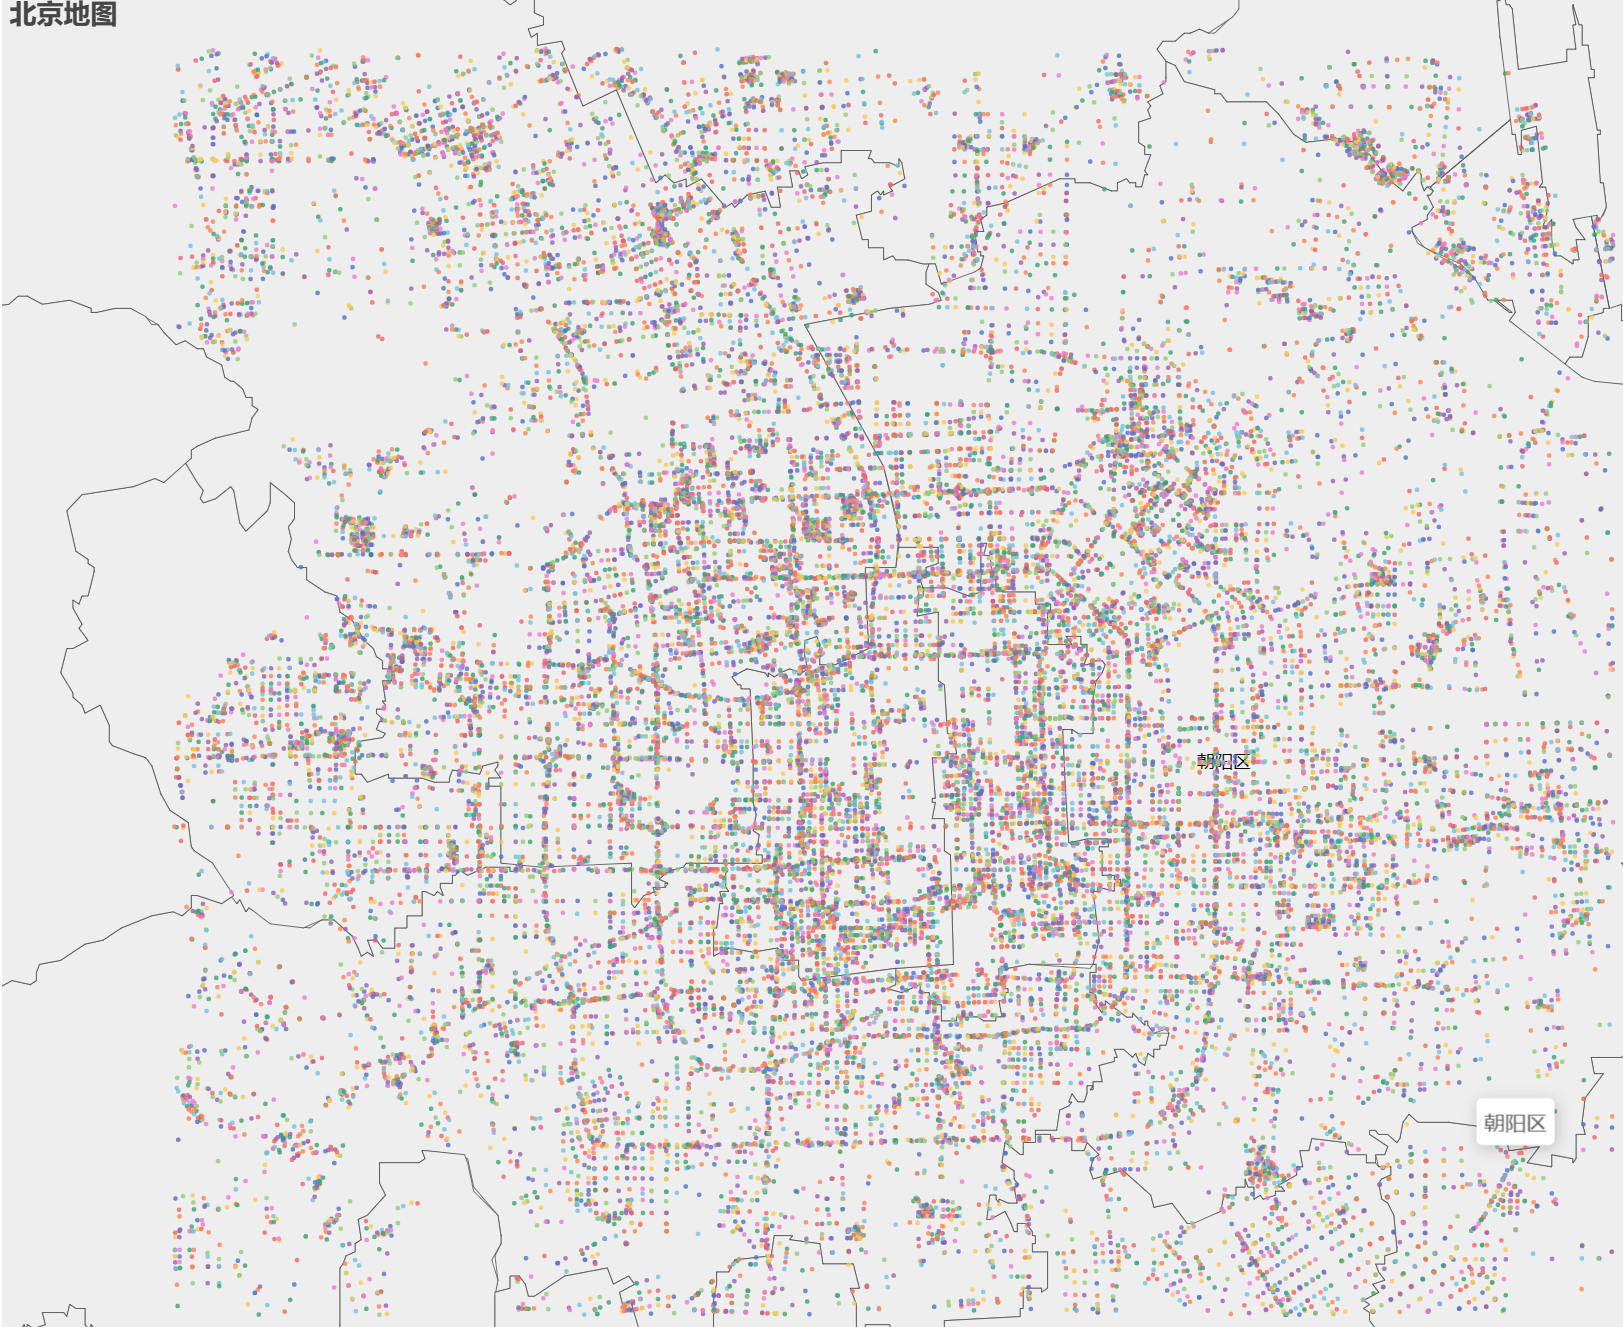
\includegraphics[width=10cm,height=7.5cm]{北京地图初始版.png}
    \caption{All Vertices Shown on the Map of Beijing}
\end{figure}
\indent We discovered that many points are located along the tracks of public transportation lines and residential areas, which aligns with our general knowledge.\\
\indent We then proceed to process the given edge values in the question. We noticed that among the provided edges, there are some instances where the length of certain edges \textbf{appears twice and is inconsistent}. We believe that this portion of the data is erroneous. Therefore, when using the data in practice, we only consider the length of the edge as it appears for the first time and remove any other erroneous data.There were \textbf{a total of 72156 edge length data} in the question, and after processing, we are \textbf{left with 71461 valid data}.\\
\indent We also analyzed the given path data in the question. For each path, we incremented the usage count of each edge by 1. We traversed all the paths, summed up the usage counts of all edges, and plotted a graph showing the proportion of edge usage counts. The figure is shown below, where the vertical axis represents the proportion and the horizontal axis represents the usage count of the edges:
\begin{figure}[H]%插入图片:次数分布
    \centering
    \subfigure[Probability Distribution Graph of  All Usage Counts ]{
    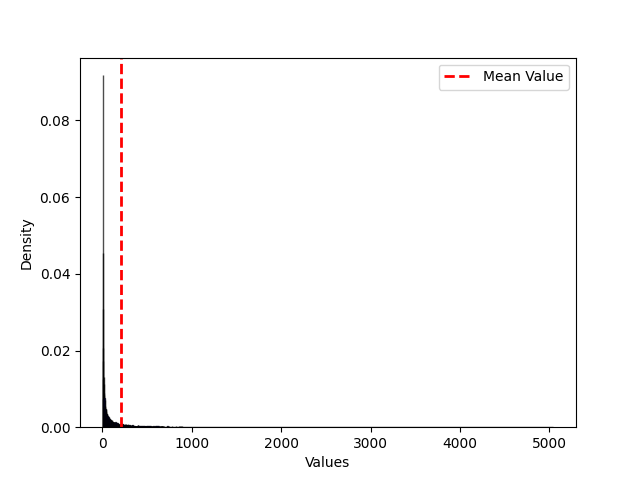
\includegraphics[width=6cm,height=4.5cm]{次数分布-总体.png}}
    \subfigure[Probability Distribution Graph of  Partial Usage Counts]{
        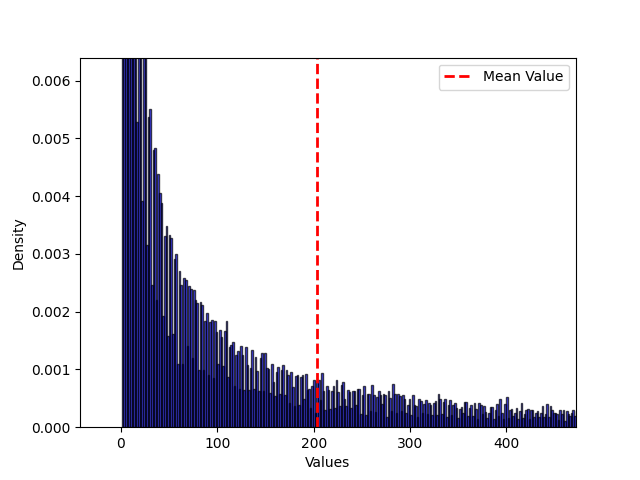
\includegraphics[width=6cm,height=4.5cm]{次数分布_局部.png}}
    \caption{Histogram of Usage Counts Frequency Distribution}
\end{figure}
\indent We found that the majority of edges have usage counts concentrated within 50 times or less. However, there is still a significant portion of edges that have usage counts exceeding 200. We believe that the more an edge is used, the more preferred it is by customers. Consequently, the importance of such an edge also increases. This will be taken into account because it influences our calculation of the road importance indicator.\\
\indent Finally,we use the valid vertices and edges to make an gragh G for case 1. Now we begin to use the graph G to construct models. 

%%%%%%%%%%%%%%%%%%%%%%%%%%%%%%%%%%%%%%%%%%%%%%%%%%%%%%%%%%%%%%%%%%%%%%%%%%%%%%%%%%%%
\subsection{Calculating the SIM Value of Case 1}
%第三小节:计算案例1中的SIM值

\indent\indent To calculate the value of SIM in Case 1, we utilize \textbf{the Dijkstra's algorithm} to compute the shortest path for each pair of starting and ending points. Since the SIM value requires counting the number of shortest paths and the total number of paths, we use a program to calculate the total number of paths visited. While traversing each path, we also record its length. Then, in combination with the Dijkstra's algorithm, we verify whether the path is indeed the shortest path for the given pair of starting and ending points. \\
\indent Dijkstra's algorithm is an algorithm used to find the shortest path from a single source node in a weighted directed or undirected graph. The goal of the algorithm is to find the shortest paths from the source node to all other nodes. It starts from the source node and gradually expands to other nodes by continuously selecting the node with the current shortest path to update the shortest paths and distances.\\
\indent The time complexity of the algorithm depends on the size of the graph and is typically $O(V^2)$, where V is the number of nodes in the graph. When using a priority queue data structure to optimize the algorithm implementation, the time complexity can be reduced to $O((V + E)logV)$, where E is the number of edges in the graph. In our actual computation process, we found that the former time complexity is too high, so we adopted \textbf{the priority queue optimization algorithm} to reduce the time complexity.\\
\indent We know that using Dijkstra's algorithm, we can calculate the shortest paths from a single starting point to all other points in one go. However, the paths provided in the question are in a disorderly sequence. In order to further reduce the time complexity, we \textbf{sorted the paths in the file in ascending order based on the numbers of the starting and ending points}. Moreover, for all paths with the same starting point, we only called the algorithm once and used an array to store the shortest path lengths from that point to all other points. This significantly reduced the time complexity.\\
\indent For example, after sorting the starting and ending point numbers in ascending order, we found a total of 64 paths with a starting point of 2. If we use the optimized algorithm, we only need to call the algorithm once and then access the generated array 64 times to calculate the shortest paths for these 64 sets of edges. Otherwise, if we had to re-call the algorithm for each path separately, the time consumption would be significant. Our basic approch is as follows:\\
\begin{figure}[H]%插入图片:dijkstra算法优化前后对照
    \centering
    \subfigure[Before Optimization]{
        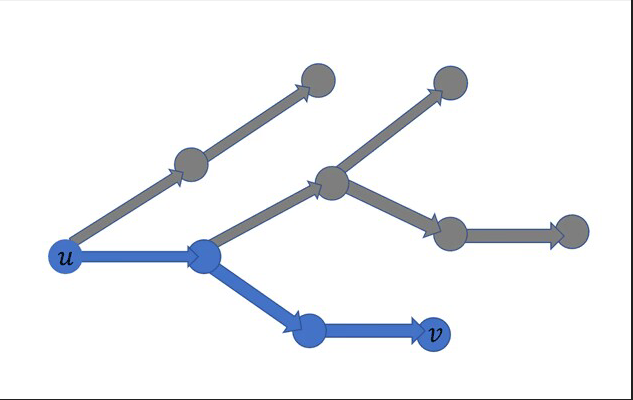
\includegraphics[width=8cm,height=6cm]{dijkstra优化前.png}}
    \subfigure[After Optimization]{
        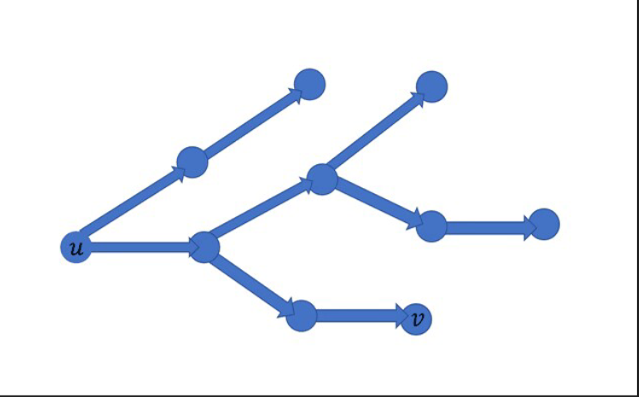
\includegraphics[width=8cm,height=6cm]{dijkstra优化后.png}}
    \caption{Basic approach of Our Optimization to the Dijkstra Algorithm}
\end{figure}
\indent When we iterate over each i-th path, we denote whether this path is the shortest path between the starting point and ending point of the group as \textbf{$a_i$}. If it is, the value is 1; otherwise, it is 0. This is represented by the following equation:\\
\[%插入公式
    a_i=
    \left\{
        \begin{array}{ll}
            1, \text{it is the shortest path}\\
            0, \text{otherwise}
        \end{array}
        \right.
\]
\indent We define \textbf{$\alpha$ as the number of paths in the provided file's paths that satisfy the shortest path condition}. The calculation formula for $\alpha$ is as follows:
\begin{equation}
    \alpha=\sum_{i=1}^{n}a_i
\end{equation}
\indent  So, the value of SIM can be obtained from the following equation:
\begin{equation}
    SIM=\frac{\alpha}{A}
\end{equation}
\indent We define \textbf{$A$ as the sum of all the numbers of paths}. And we import the data that has been processed into the program and obtain the changes in SIM as the program sequentially imports paths according to the order of the provided files in the question. The change curve is as follows:\\
\begin{figure}[H]%插入图片:遍历path过程中SIM实时变化
    \centering
    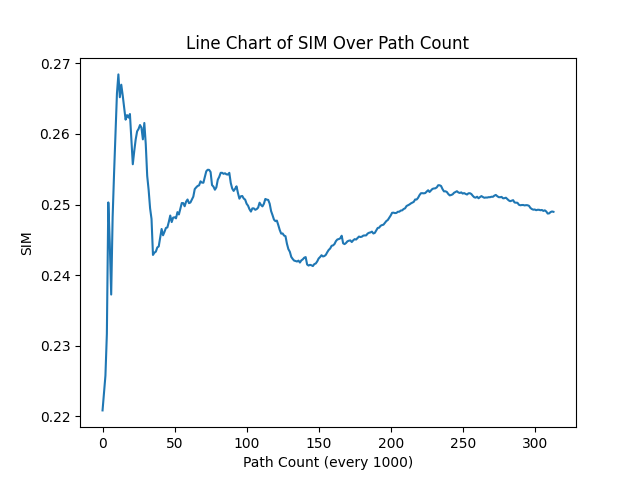
\includegraphics[width=10cm,height=7.5cm]{Figure_1-1.png}
    \caption{Line Chart of SIM Over Path Count}
\end{figure}
\indent According to Figure 6, we can draw the conclusion that the value of SIM oscillates as the data is read in and eventually stabilizes around 0.25.  And \textbf{the final value of SIM in Case 1 is 0.248971}.\\
\indent Then, we use this model, which is capable of calculating SIM values, to compute the SIM value for the edge weight corresponding to Table 1 in the first task. The result is 0.75, which matches the result we obtained through iterative attempts. This indicates that our first task result is correct, and the model is indeed capable of effectively computing SIM values.

%%%%%%%%%%%%%%%%%%%%%%%%%%%%%%%%%%%%%%%%%%%%%%%%%%%%%%%%%%%%%%%%%%%%%%%%%%%%%%%%%%%%
\subsection{Model of Maximizing the SIM in Case 1}
%第五小节:建模指标和过程

\subsubsection{Simulated Annealing Algorithm}
%退火算法

\indent\indent Simulated Annealing Algorithm is a global optimization algorithm commonly used to solve complex combinatorial optimization problems. The algorithm simulates the behavior of molecular motion during the annealing process of a solid, accepting solutions that are worse than the current solution with a certain probability to avoid getting trapped in local optima and to search for the global optimum.\\
\indent The basic idea of the Simulated Annealing Algorithm originates from the physical phenomenon observed in the annealing process of solids. In the annealing process, by gradually lowering the temperature, atoms or molecules gain enough energy to escape from states with local energy minima, providing an opportunity to reach the global energy minimum state.\\
\indent The Simulated Annealing Algorithm is typically used to compute the minimum value of an objective function. However, in our case, we need to find the maximum value of the objective function SIM. Therefore, some adjustments need to be made to the algorithm.\\
\indent When making the logical decision of whether to accept a new SIM value, we modify the acceptance criterion. If the new SIM value is greater than the current SIM value, we accept the new SIM value with a probability of $100\%$. If the new SIM value is smaller than the current SIM value, the original algorithm would result in an exponential function with an exponent greater than 0, making the probability exceed 1. So in the expression, we add a negative sign to the exponent, as shown in the following formula:
\[%插入公式
    P_{i+1}=
    \left\{
        \begin{array}{ll}
            1, SIM_{i+1} \geq SIM_i \\
            \exp\left(\dfrac{{SIM_{i+1} - SIM_i}}{{T_{i+1}}}\right), SIM_{i+1} < SIM_i
        \end{array}
        \right.
\]
\indent \textbf{$P_{i+1}$ represents the probability of accepting a new SIM value in the first round. $SIM_i$ represents the SIM value in the i-th round, and $T_i$ represents the temperature in the i-th round}, whose expression can be written as:
\begin{equation*}
    T_i=\lambda^i \cdot T_0
\end{equation*}
\indent In the given code, \textbf{$T_0$ ,$T_{end}$ and $\lambda$ are pre-set based on actual conditions}. According to many trials, we determine \textbf{$\lambda$ as 0.9}. When $T$ reaches $T_{end}$, the annealing process will automatically terminate, and the program stops running. The current SIM value represents the final result. The following Figure shows how the simulated annealing algorithm works:\\
\begin{figure}[H]%插入图片:模拟退火的工作场景
    \centering
    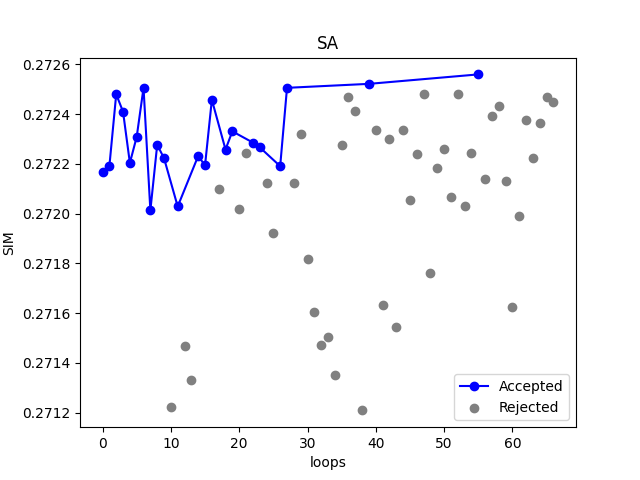
\includegraphics[width=8cm,height=6cm]{SA1-1.png}
    \caption{The curve of SIM value changes in An Annealing}
\end{figure}
\indent The blue points in the graph represent the accepted results, indicating that the new SIM value is greater than the original SIM value. The gray points represent the rejected new SIM values, indicating that the new SIM value is smaller than the original SIM value and was not accepted. From Figure 7, we can observe that the SIM value exhibits a fluctuating upward trend during this annealing process. Additionally, there are several rejections between two consecutive acceptances in order to break out of a local optimum.\\
\indent When calculating the objective function SIM, we need to compute the weights of each edge, so we need to determine the expression for edge weights. The expression for edge weights will be provided later. First, we will discuss one of the important factors in determining the weight expression, which is the importance of the roads. The next subsubsection will introduce the metric we adopted to measure the importance of roads, which is the PageRank of the edges.

\subsubsection{PageRank and Edge PageRank}
%PageRank

\indent\indent PageRank is an algorithm used to measure the importance or relevance of web pages within a network. It was developed by Google's co-founders, Larry Page and Sergey Brin. PageRank assigns a numerical value called PageRank score to each web page in the network. The score is based on the idea that important web pages are likely to receive more links from other web pages. The PageRank score of a web page is influenced by the quantity and quality of incoming links. Web pages with higher PageRank scores are considered more authoritative and are given higher priority in search engine results. The PageRank formula in a general sense is described by the following formula:
\begin{equation*}
    PR(i)=(1-\gamma)+\gamma \cdot \sum_{1}^{n} \frac{PR(j)}{deg(j)}
\end{equation*}
\indent \textbf{$PR(i)$ represents the PageRank value of webpage i, $PR(1)$ to $PR(n)$ represent the PageRank values of other webpages that link to webpage $i$, $deg(1)$ to $deg(n)$ represent the outgoing link counts from other webpages to webpage $i$, and $\gamma$ is a damping factor between 0 and 1 used to control the probability of random jumping}.\\
\indent PageRank is mostly used for assessing the importance of webpages or entire websites, and it is rarely applied to evaluate the importance of edges. Therefore, we try to utilize this algorithm to measure the frequency of road usage. \\
\indent For any arbitary graph G with vertex set V and edge set E, and for any edge e with u as the starting point and v as the endpoint, the edge PageRank value is defined as:
\begin{equation*}
    PR^{\gamma}_e(G)= \frac{1}{deg^{+}_u(G)}( \gamma\cdot\sum_{e^{\prime}\in E^-_u(G)}^{}PR^{\gamma}_{e^{\prime}}(G)+\Phi(u))
\end{equation*}
\indent \textbf{$PR^{\gamma}_e(G)$ represents the PageRank value of edge e, $deg^{+}_u(G)$ represents the size of the set of all the outgoing edges, namely the out-degree of the vertex u, $\Phi(u)$ represents a empirical formula associated with u}, and we give it \textbf{an initial value of 1} for convenience. \textbf{$\gamma$ represents a parameter. Referring to previous literature, we assign a value of 0.85 to $\gamma$}. According to the recursive formula, as an edge is traversed more frequently, the sum of the edge PageRank values of its adjacent edges increases, resulting in a higher PageRank value for that edge.\\
\indent We substituted the data for case 1 into the formula and performed the calculations. We then plotted the probability density graph of the edge PageRank values, as shown in the following figure:
\begin{figure}[H]%插入图片:PR分布
    \centering
    \subfigure[Probability Distribution Graph of  All Edge PageRank]{
    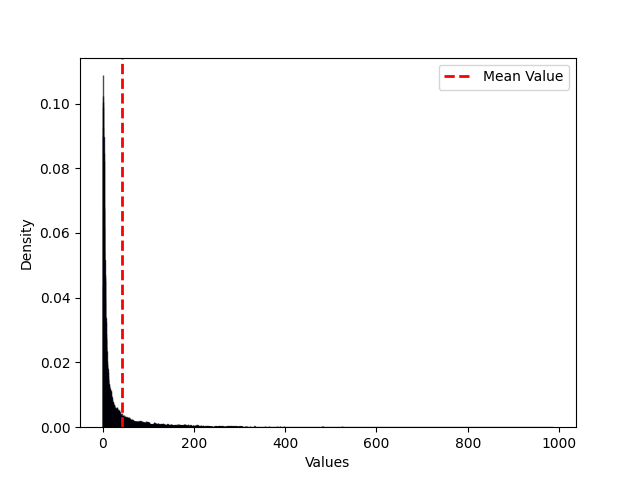
\includegraphics[width=6cm,height=4.5cm]{PR分布-总体.png}}
    \subfigure[Probability Distribution Graph of  All Edge PageRank]{
        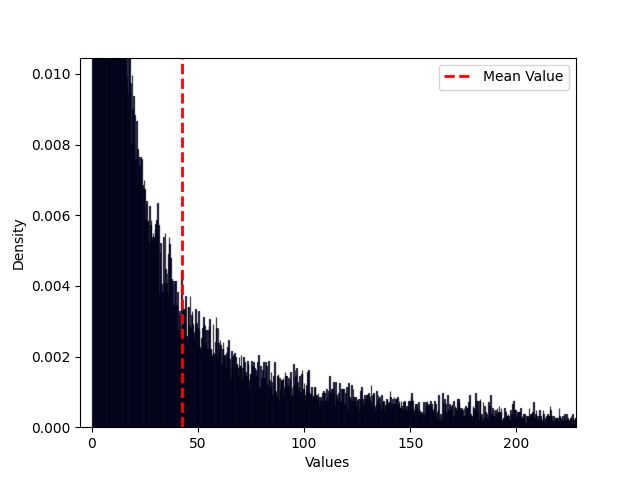
\includegraphics[width=6cm,height=4.5cm]{PR分布_局部.png}}
    \caption{Histogram of Edge PageRank Frequency Distribution}
\end{figure}
\indent The left figure represents the overall distribution of edge PageRank values, while the right figure displays the data within the range of 0 to 250 for edge PageRank values. It can be observed that the majority of edges have PageRank values below 50. However, there are also some road edges with PageRank values exceeding 100 or even 200, indicating that using edge PageRank to determine the importance of roads exhibits significant differentiation and reliability.

\subsubsection{The Straight-line Distance and Length of Roads}
%distance

\indent\indent To incorporate the length of the road traveled, we consider both the road length and the straight-line distance between the starting point and the endpoint of the road when calculating the weight. This allows us to better capture potential user preferences for taking longer routes. Therefore, we define the length of road e as $length_e$ and the straight-line distance between the starting point and endpoint as $dist_e$.\\
\indent The data for the road length has been provided in the question and processed accordingly. However, to calculate the straight-line distance of the road, we need to utilize the given longitude and latitude coordinates. For an edge $e$, given the latitude and longitude coordinates of its starting point $u$ and endpoint $v$, the calculation formula of $dist_e$ is as follows:
\begin{equation*}
    dist_e=1000\times \sqrt{85.714\times (lon_u-lon_v)^2+78.125\times (lat_u-lat_v)^2}
\end{equation*}
\indent In the formula above, \textbf{$lon_u$ and $lon_v$ represent the longitudes of the starting point and endpoint of road e, respectively}. \textbf{$lat_u$ and $lat_v$ represent the latitudes of the starting point and endpoint of road e  respectively}. The straight-line distance between the two locations can be obtained by calculating the weighted sum of these values.


\subsubsection{Initial Model}
%建立最初的模型

\indent\indent Now we can attempt to write the expression for the weight of an edge, denoted as $\omega$:
\begin{equation*}
\omega_e=\frac{\xi}{PR^{\gamma}_e(G)}+\zeta length_e+\eta dist_e
\end{equation*}
\indent \textbf{$PR^{\gamma}_e(G)$ is the PageRank value of edge e, $length_e$ is the length of edge e, and $dist_e$ is the straight-line distance between the starting point and the endpoint of edge e}. $\xi$, $\zeta$, and $\eta$ are constants that need to be solved using the simulated annealing algorithm.\\
\indent We utilize the simulated annealing algorithm to calculate three parameters that determine the weights, using the SIM value as the objective function, and record \textbf{the maximum SIM value is 0.273278}.

%%%%%%%%%%%%%%%%%%%%%%%%%%%%%%%%%%%%%%%%%%%%%%%%%%%%%%%%%%%%%%%%%%%%%%%%%%%%%%%%%%%%
\subsection{Model Optimizing}
%建模优化过程

\subsubsection{Data Re-mining}
%数据的再挖掘

\indent\indent When we constructing the models, we also investigated the relationship between the PageRank value of each edge and the connection between its starting point and endpoint. The scatter plots are shown below in the respective figures: 
\begin{figure}[H]%插入图片:PR与uv的关系
    \centering
    \subfigure{
    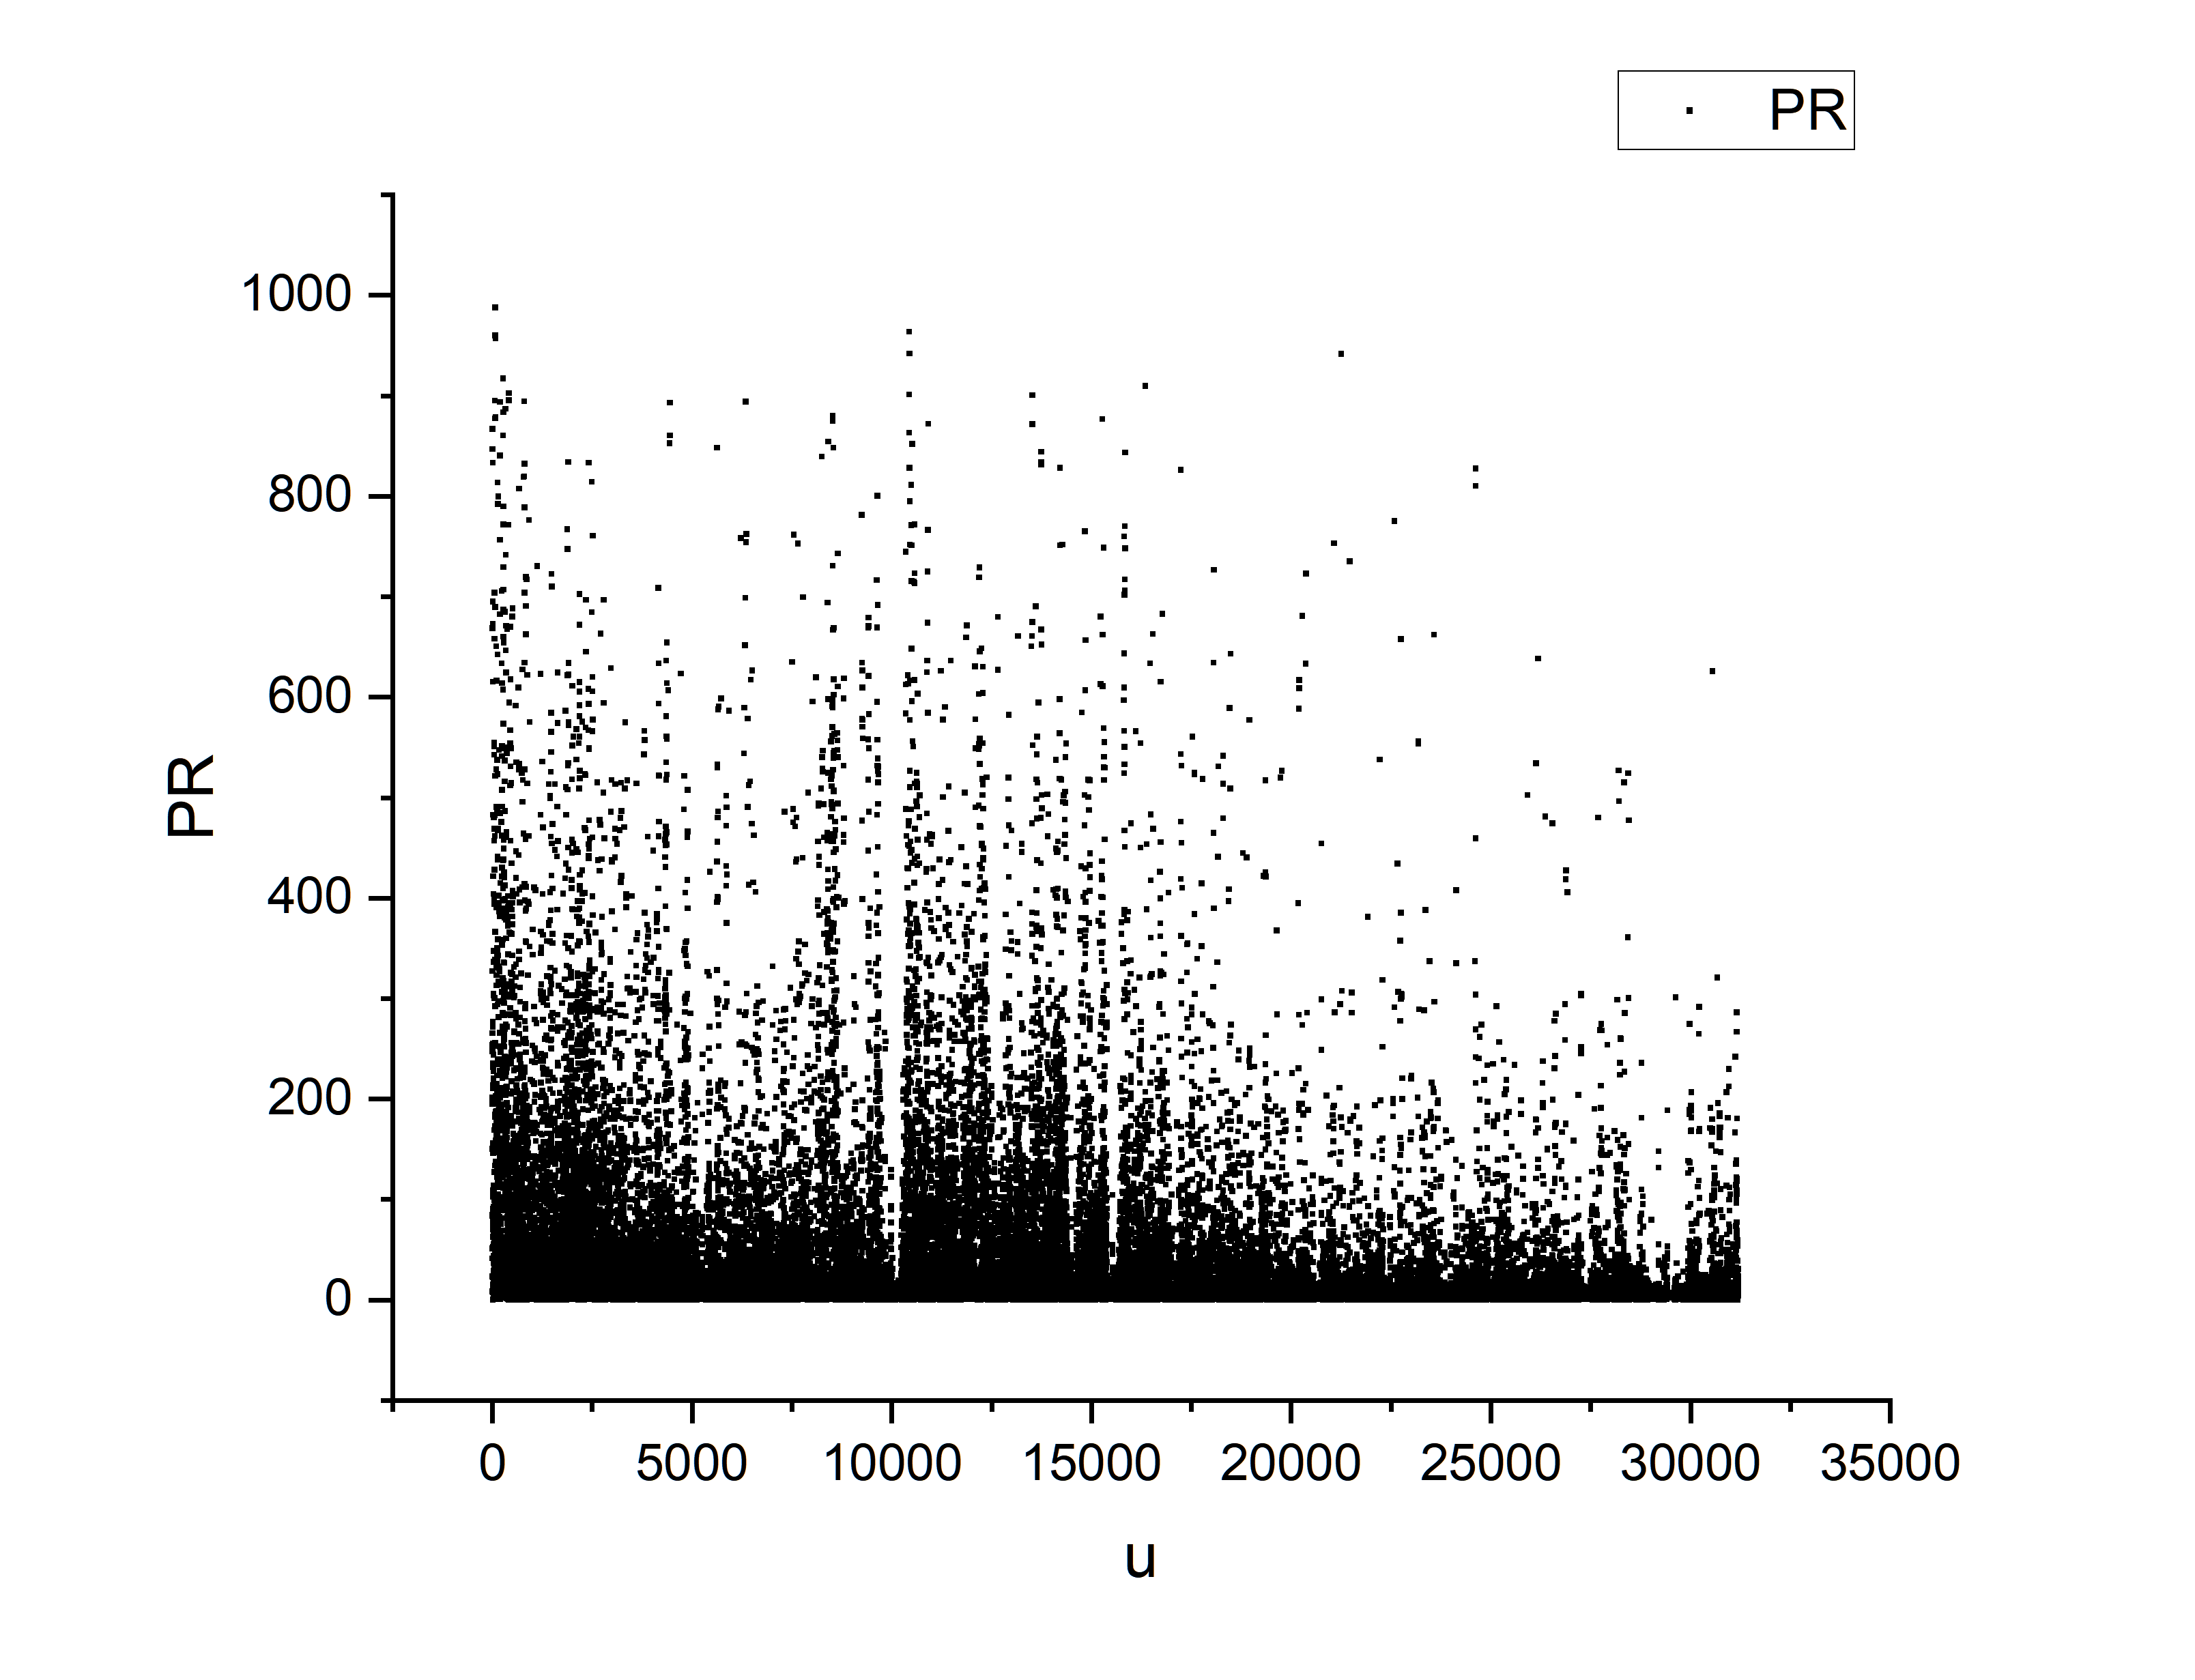
\includegraphics[width=6cm,height=4.5cm]{PR与u的关系.png}}
    \subfigure{
    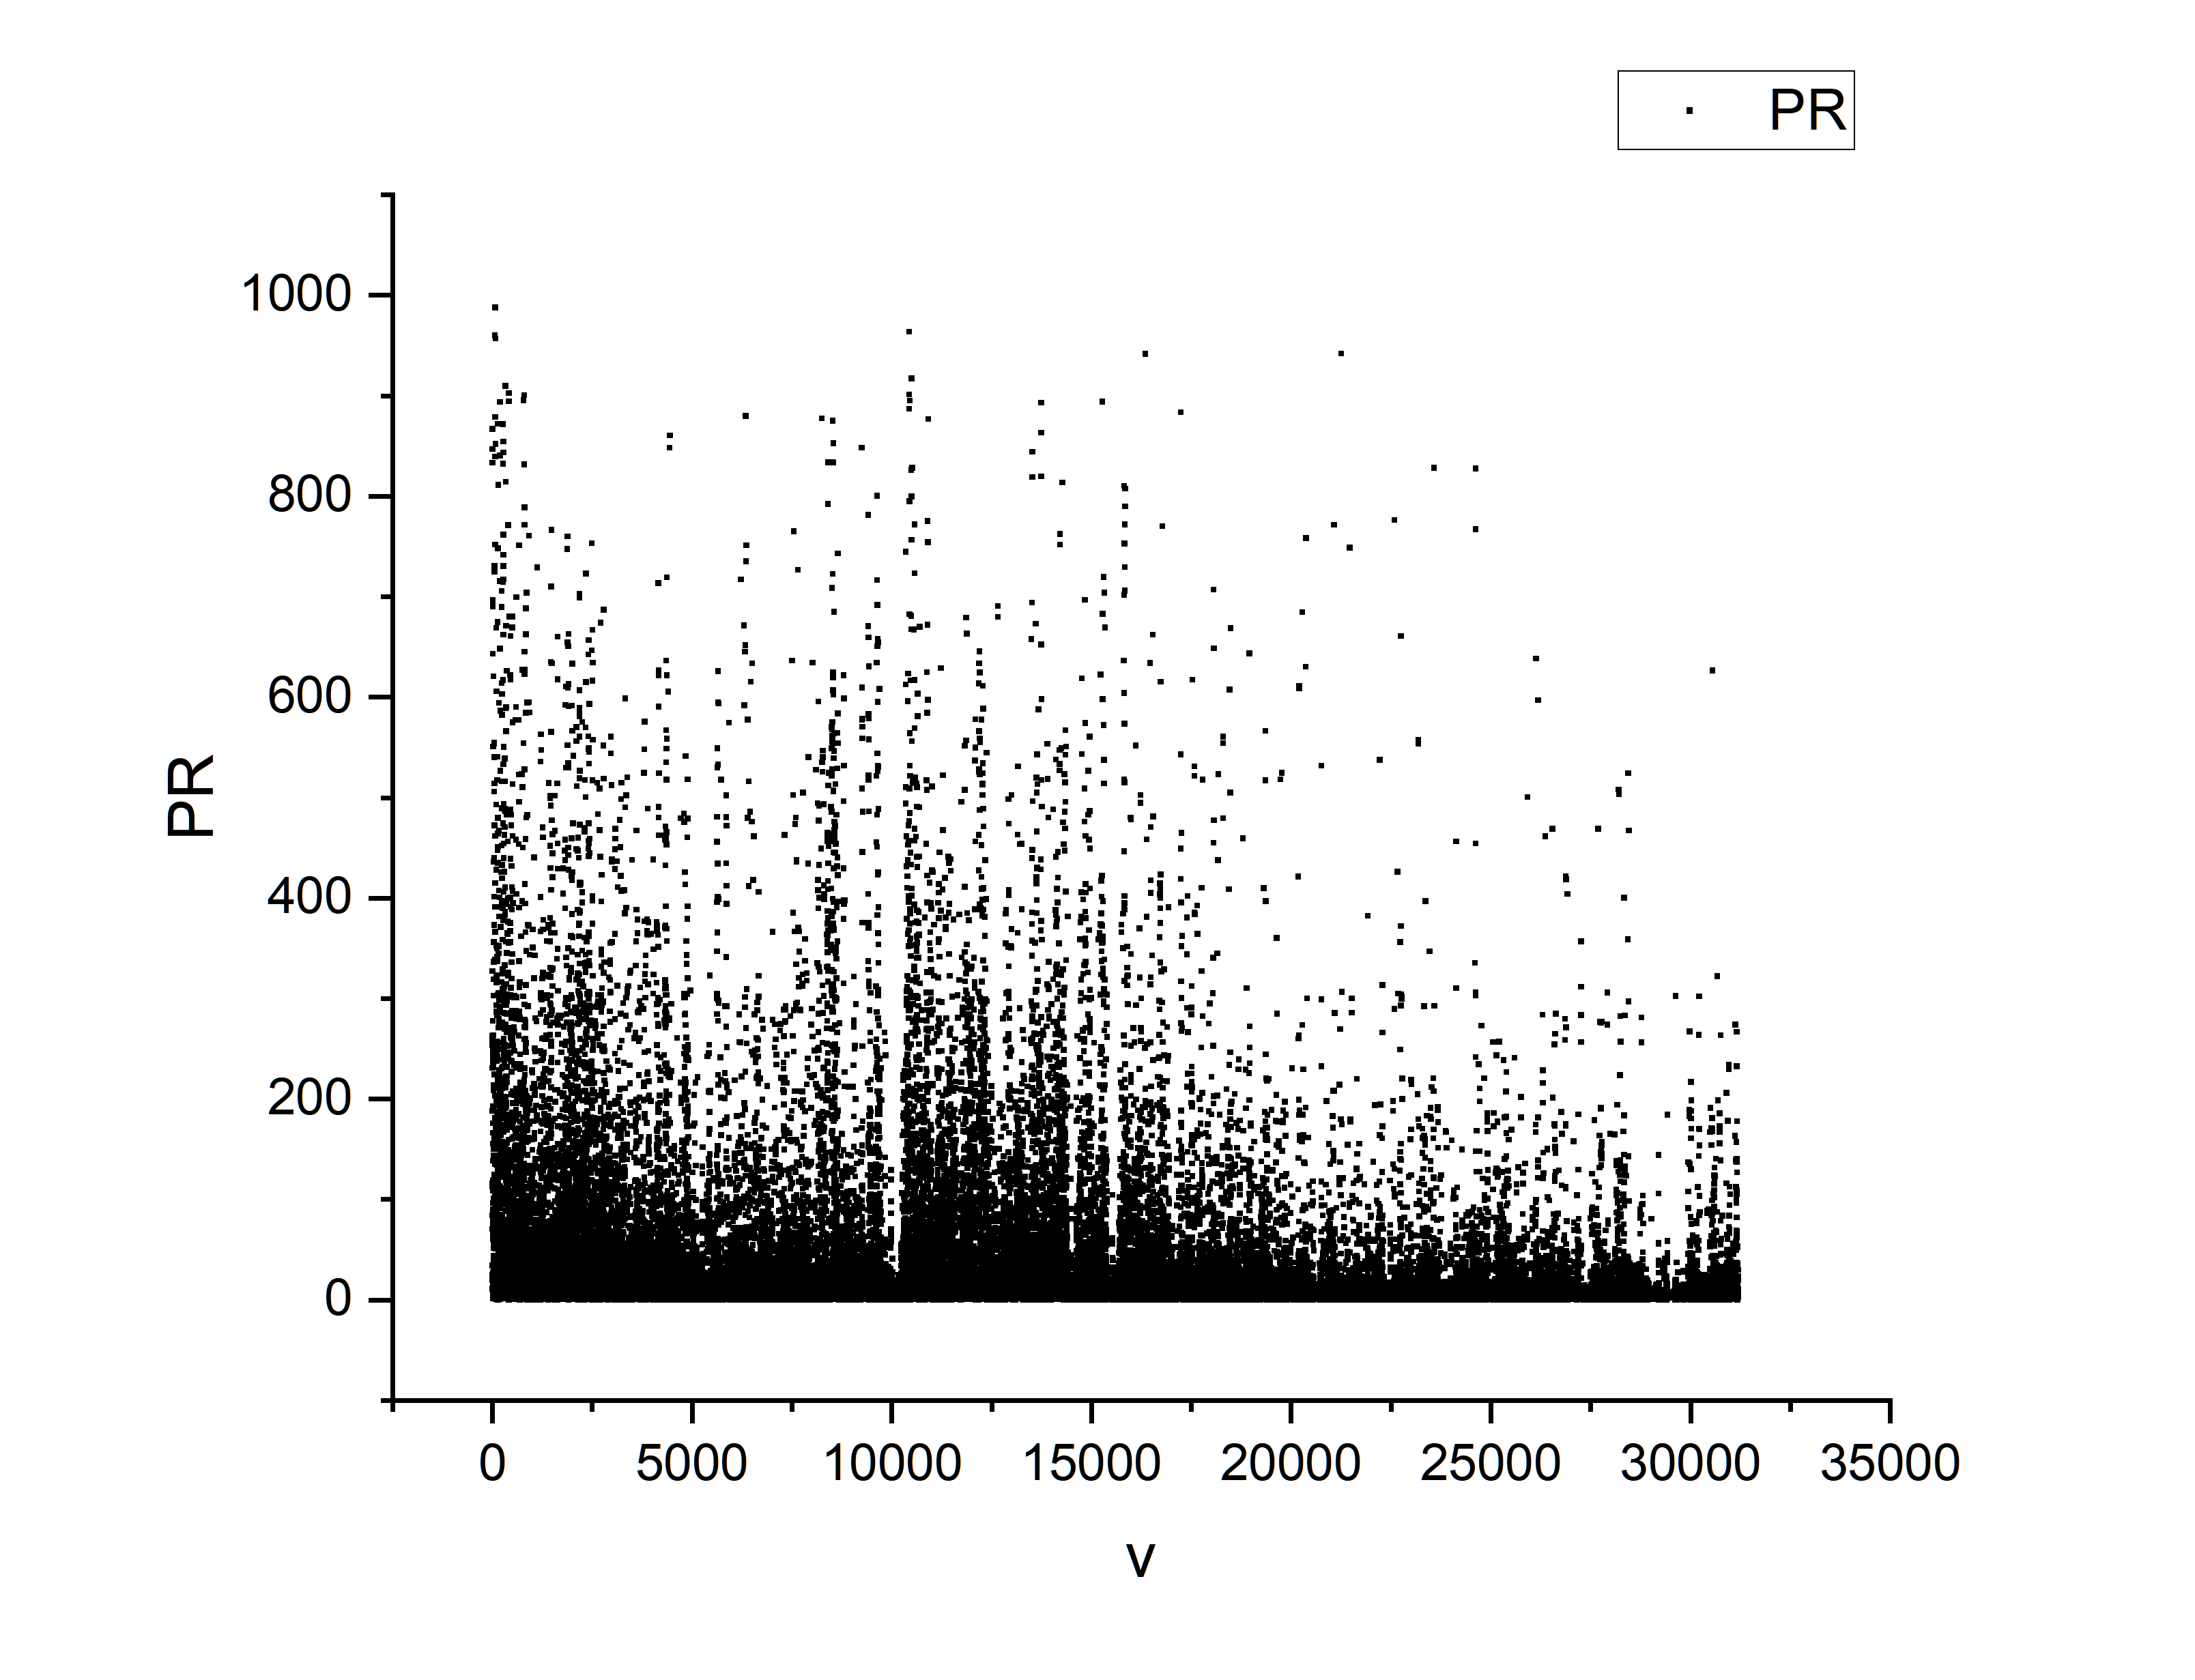
\includegraphics[width=6cm,height=4.5cm]{PR与v的关系.png}}
    \caption{The Relationship between PR and u/v}
\end{figure}
\indent From the two figures above, we can deduce there is \textbf{a significant "gap" in the PageRank values when the starting point or endpoint is around 10000}. Therefore, we believe it is necessary to investigate the relationship between the locations in this area and the notably lower PR values. As a result, we have marked the points from 9800 to 10200 on the map of Beijing, as shown in the figure below.
\begin{figure}[H]%插入图片:10000左右的点进行对照
    \centering
    \subfigure{
    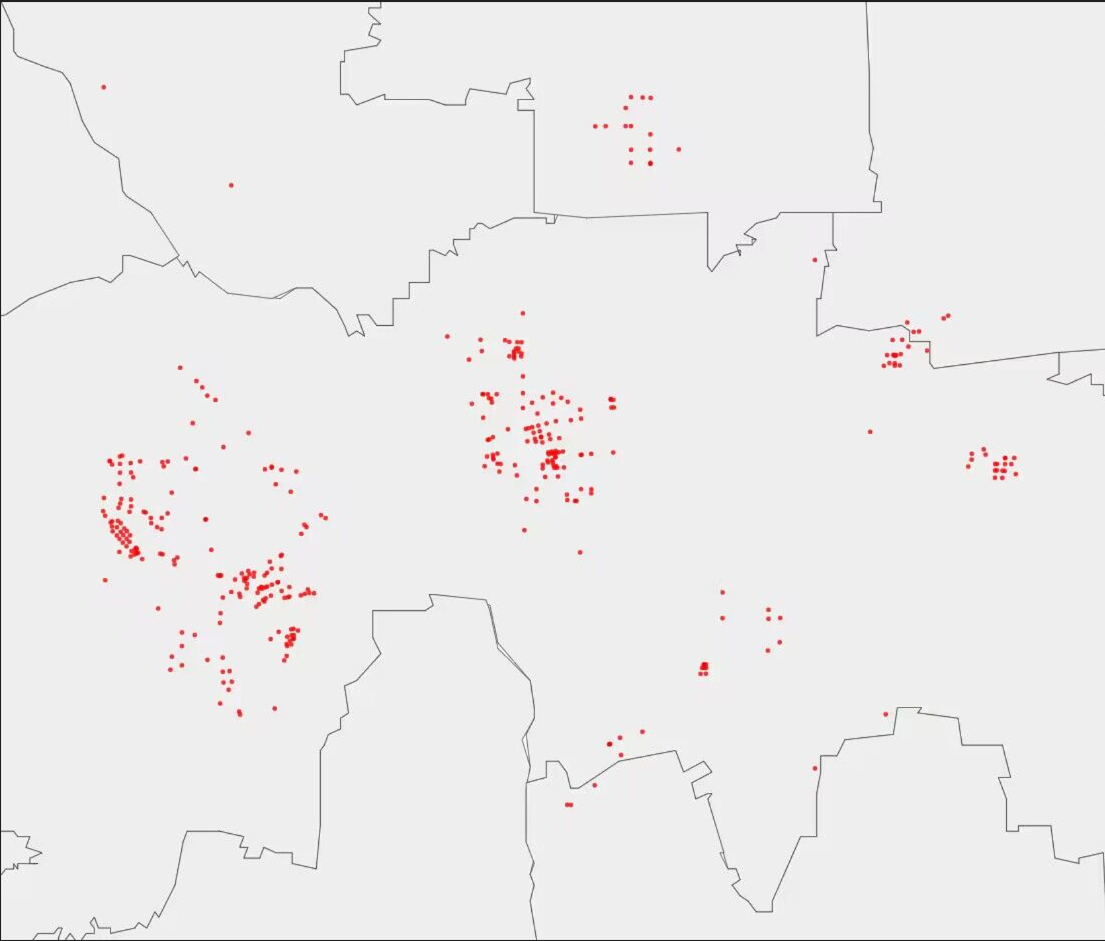
\includegraphics[width=6cm,height=4.5cm]{10000左右点.png}}
    \subfigure{
    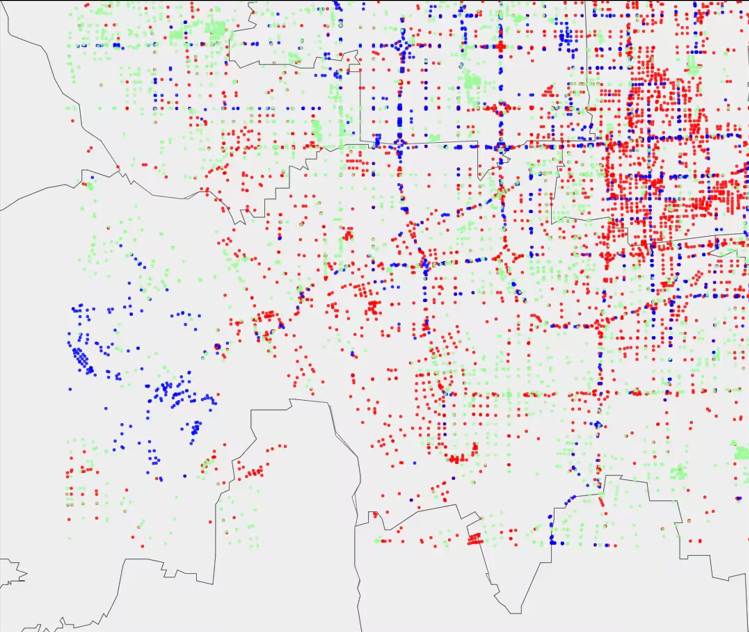
\includegraphics[width=6cm,height=4.5cm]{10000左右点对照.png}}
    \caption{The Relationship between PR and u/v}
\end{figure}
\indent From the figure, it can be observed that this subset of points is concentrated \textbf{on the southwest edge of the Beijing map}. Therefore, we believe that these points need to be treated differently and undergo special handling during the subsequent model optimization process.\\
\indent At the same time, in Figure 9 the edge weights of points below 10000 are generally higher. The points ranging from 10000 to 20000 having high edge weights as well. So we proceed to mark points in different ranges with different colors and redraw the distribution of data points on the map. Points with sequence numbers less than 10000 will be shown in red, points with sequence numbers between 10000 and 20000 will be shown in blue, and points exceeding 20000 will be shown in green. The representation of all data points on the map of Beijing is shown with specific color in the figure below:
\begin{figure}[H]%插入图片:数据点在地图上以不同颜色展现 This suggests that people are mostly active within the fourth ring road. These roads are used more frequently, hence having higher edge weights. On the other hand, less frequented and more remote roads have lower edge weights, aligning with the common preference of avoiding longer routes.
    \centering
    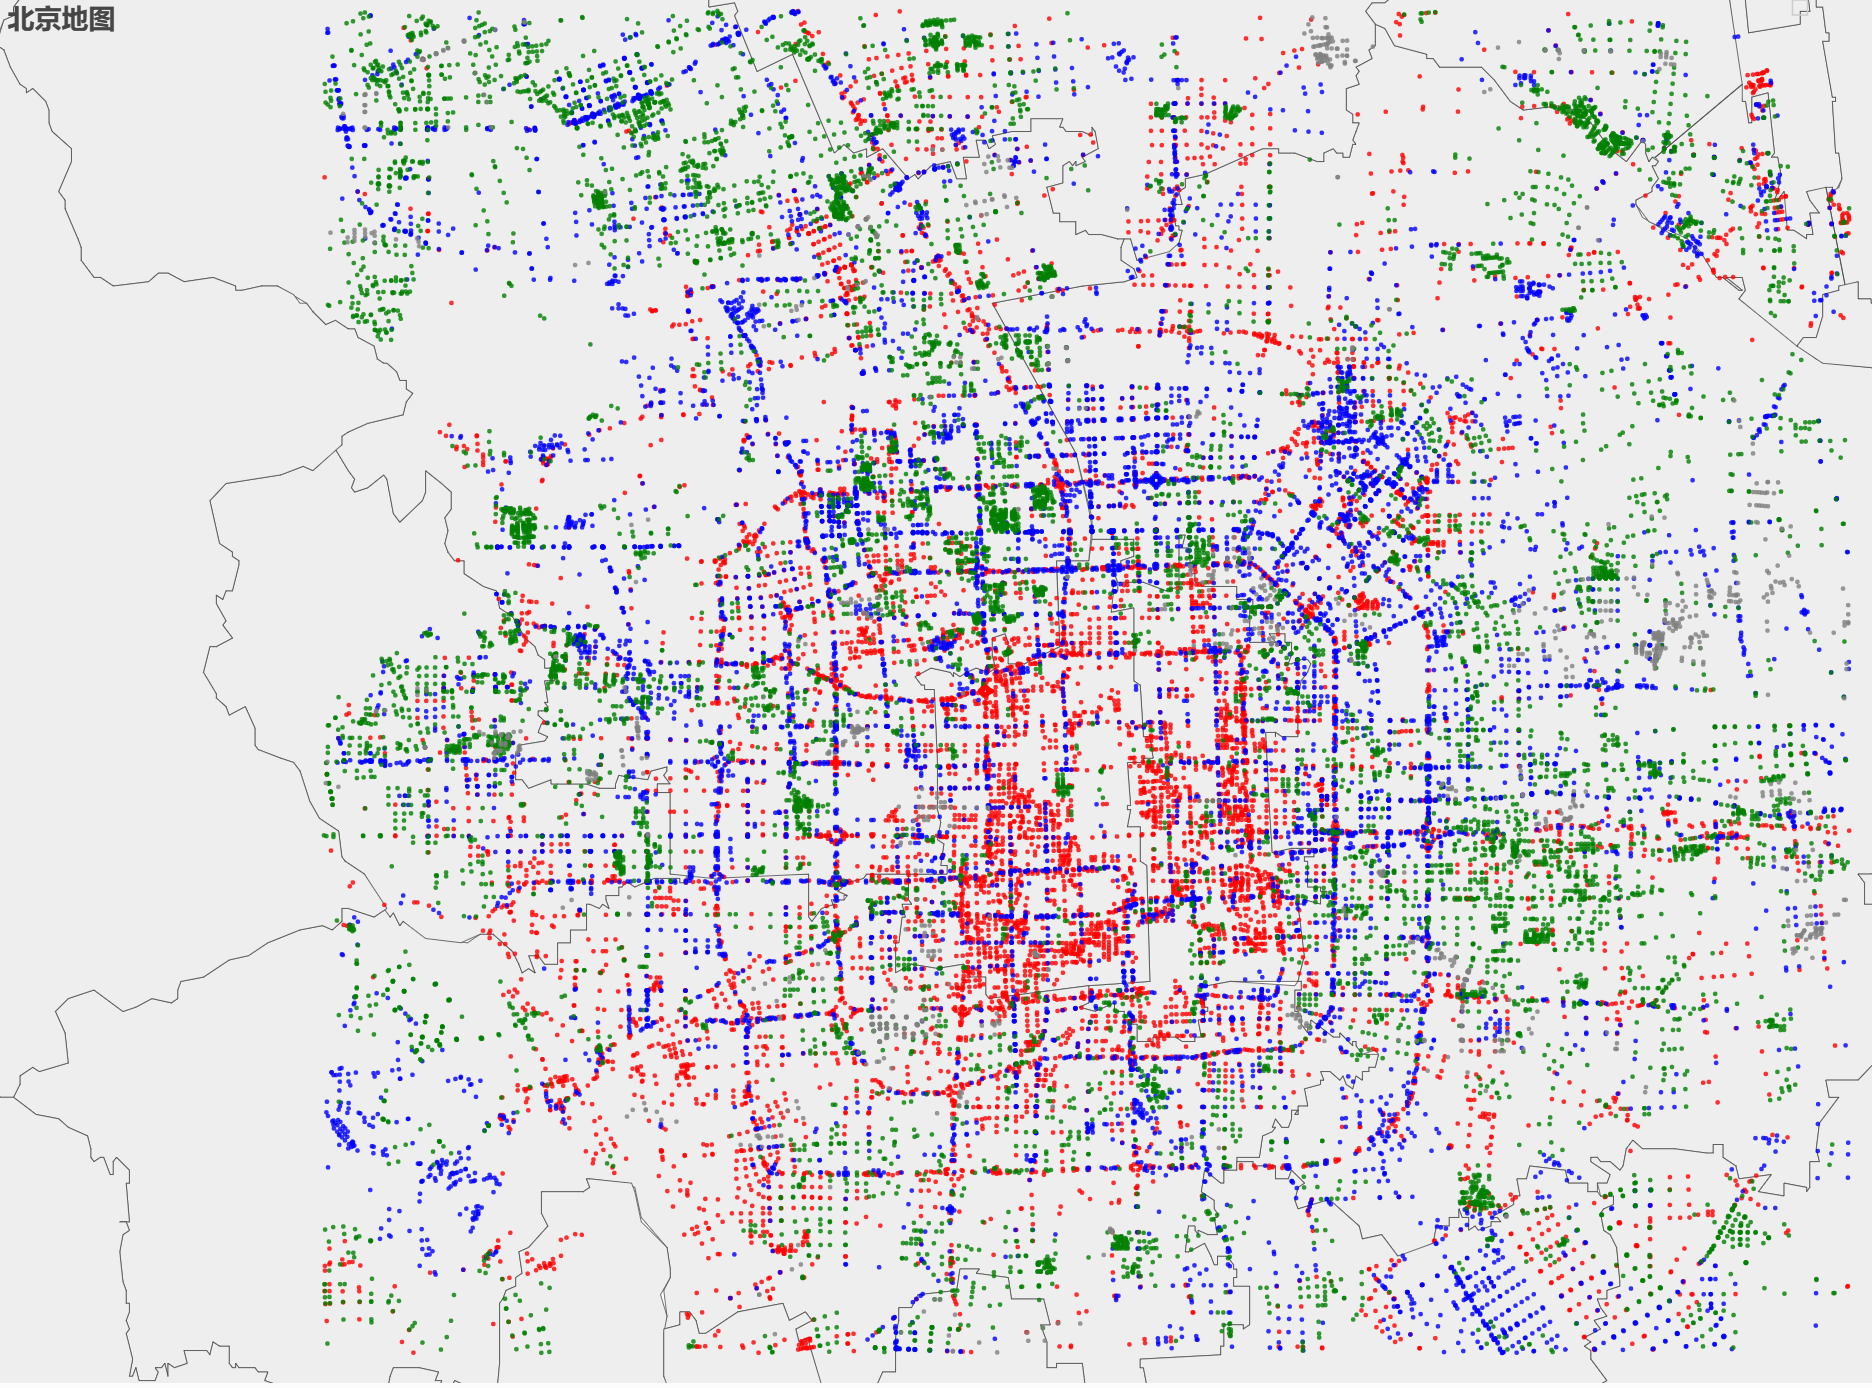
\includegraphics[width=8cm,height=6cm]{北京地图.png}
    \caption{All the Vertices Shown on the Map}
\end{figure}
\indent We discover a strong regularity in the distribution of the points: the red points are concentrated in the middle, while the blue points are primarily concentrated between the third and fourth ring roads. The distribution pattern of the green points are distributed on the outer side overall, which means points beyond 20000 do not exhibit a clear distribution pattern, but they are generally located in more remote areas, with lower corresponding edge pageranks.\\
\indent Additionally, on the map, it is evident that there is a higher concentration of people traveling to important facilities or buildings such as subway lines, residential areas, and tourist attractions. To better illustrate the relationship between the distribution of the points and the railway transportation layout in Beijing, we have registered the previous map with the Beijing transportation network map. We have adjusted the transparency to enhance clarity, as shown in the following figure:
\begin{figure}[H]%插入图片:数据在北京交通图上展现
    \centering
    \includegraphics[width=8cm,height=6cm]{覆盖北京地图.png}
    \caption{Vertices Shown on the Transportation Network of Beijing.}
\end{figure}

\indent After the aforementioned data analysis, we have discovered a strong correlation between \textbf{the index of a point and its location}. Additionally, certain specific points represent special locations. Therefore, we believe that modifying $PR^{\gamma}_e(G)$ based on the index of a point can be beneficial.\\
\indent At the same time, the third parameter $\eta$ of the initial model seemes to \textbf{have a relatively minor impact on the SIM value}, as the following figure shows:
\begin{figure}[H]%插入图片:第三个参数没啥用
    \centering
    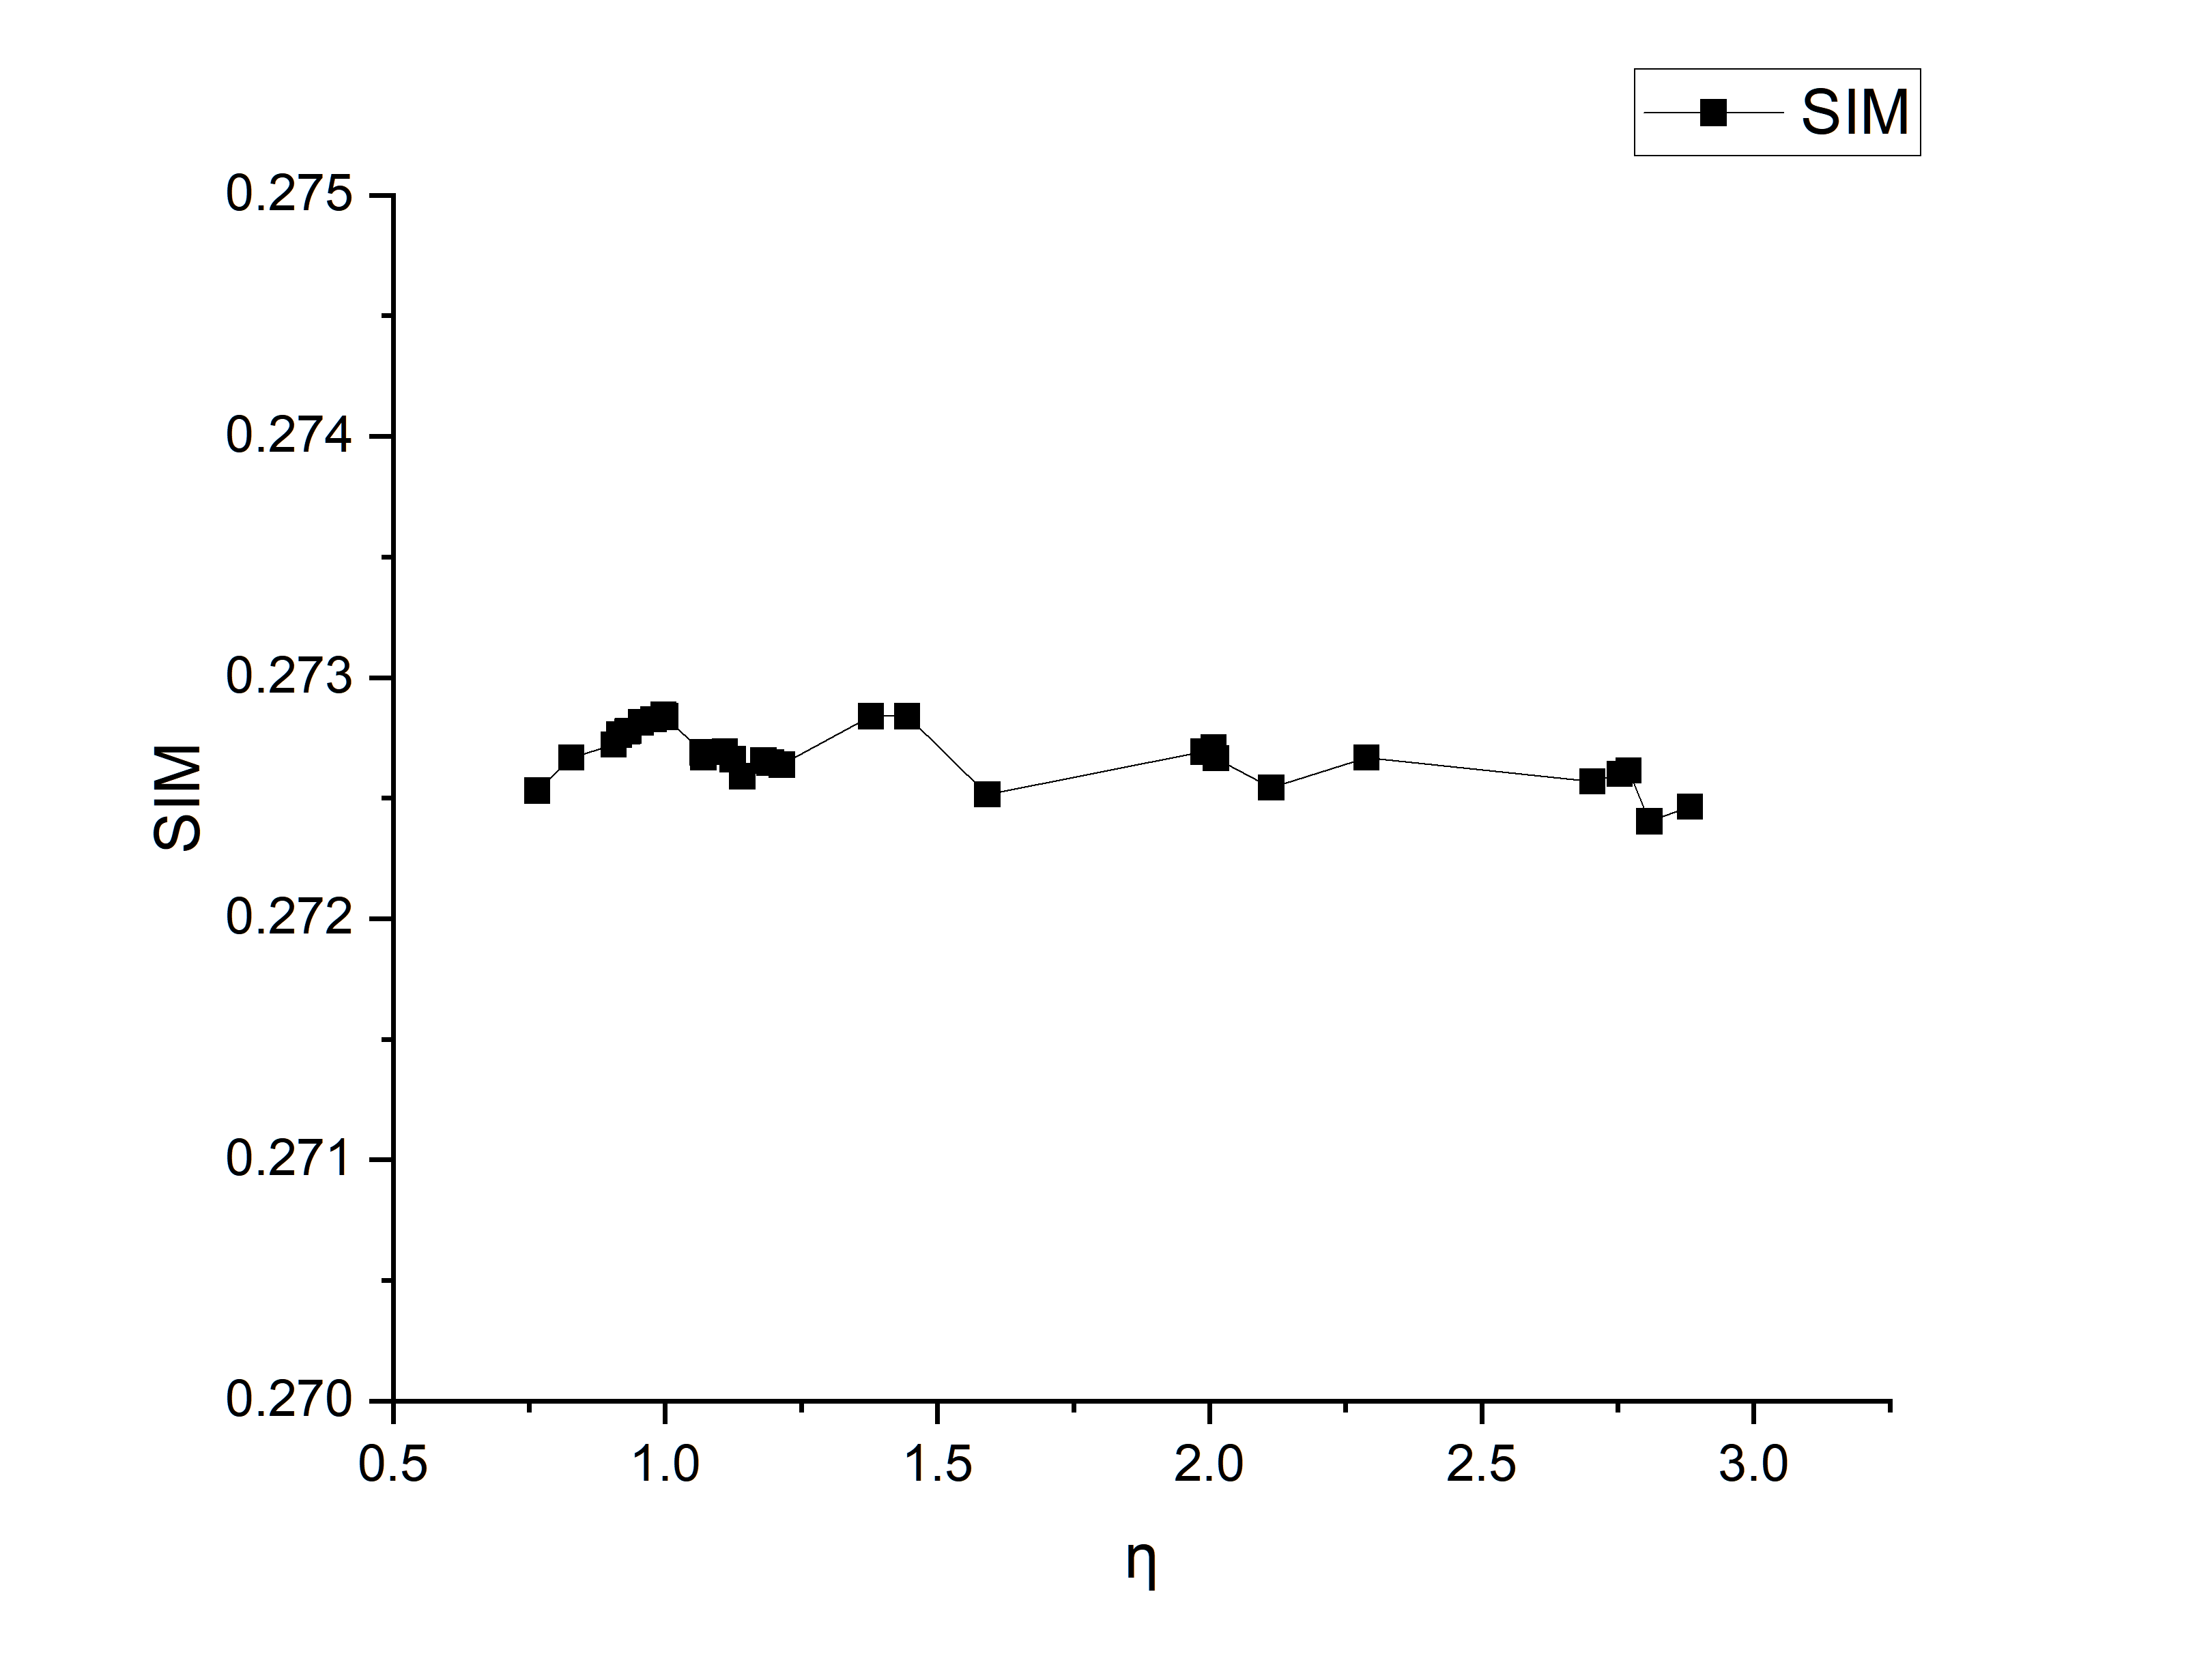
\includegraphics[width=8cm,height=6cm]{SIM-c.png}
    \caption{The Relationship between SIM and $\eta$}  
\end{figure}
\indent From the Figure, we can observe that when the two parameters remain constant, the impact of $\eta$ on the model results is not significant. The latitude and longitude coordinates used in the $dist_e$ function can be represented by the index of the points. Therefore, we will remove the third parameter from the model and optimize the calculation method for $\Phi(u)$ of the $PR^{\gamma}_e(G)$ .

\subsubsection{Model Adjusting}
%调整模型

\indent\indent By removing the third parameter and only keeping A and B, we obtain the following expression for the weight $\omega_e$:
\begin{equation*}
    \omega_e=\frac{\xi}{PR^{\gamma}_e(G)}+\zeta length_e+C 
\end{equation*}
\indent The expression of $\Phi(u)$ in $PR^{\gamma}_e(G)$ is as shown in the following formula:
\begin{equation*}
    \phi(u)=
    \left\{
        \begin{array}{ll}
            2, 0 \leq u \textless 4800 \\
            1, 4800 \leq u \textless 9800\\
            0.02, 9800 \leq u \textless 10200\\
            1.4, 10200 \leq u \textless 16000\\
            1.4e^{1.355-8.471\times 10^{-5} u}, 16000 \leq u \textless 31198\\
        \end{array}
        \right.
\end{equation*}
\indent The expression in the last part is obtained by fitting a curve to the points in the right section of Figure 9. \\
\indent \textbf{The maximum SIM value achieved by our optimized model is 0.298223}, while the maximum SIM value of the original model is 0.273278. \textbf{The optimization rate is calculated as 9.128\%}.

\subsection{Analysis and Comparison}
% 结合案例来说明我们计算weight的有效性

\indent\indent From the calculations in the previous sections, it can be observed that the maximum SIM value obtained by considering the path length as the weight is 0.248971. The maximum SIM values obtained by the original and optimized models, which calculate the weights differently, are 0.273278 and 0.298223, respectively. The optimization rates are \textbf{9.76298\% and 19.7822\%}, respectively.\\
\indent To better illustrate the difference between our method of calculating edge weights and the length of the edges, we have plotted a scatter plot showing the relationship between edge weights and lengths, as shown in the following figure:
\begin{figure}[H]%插入图片:weight-length
    \centering
    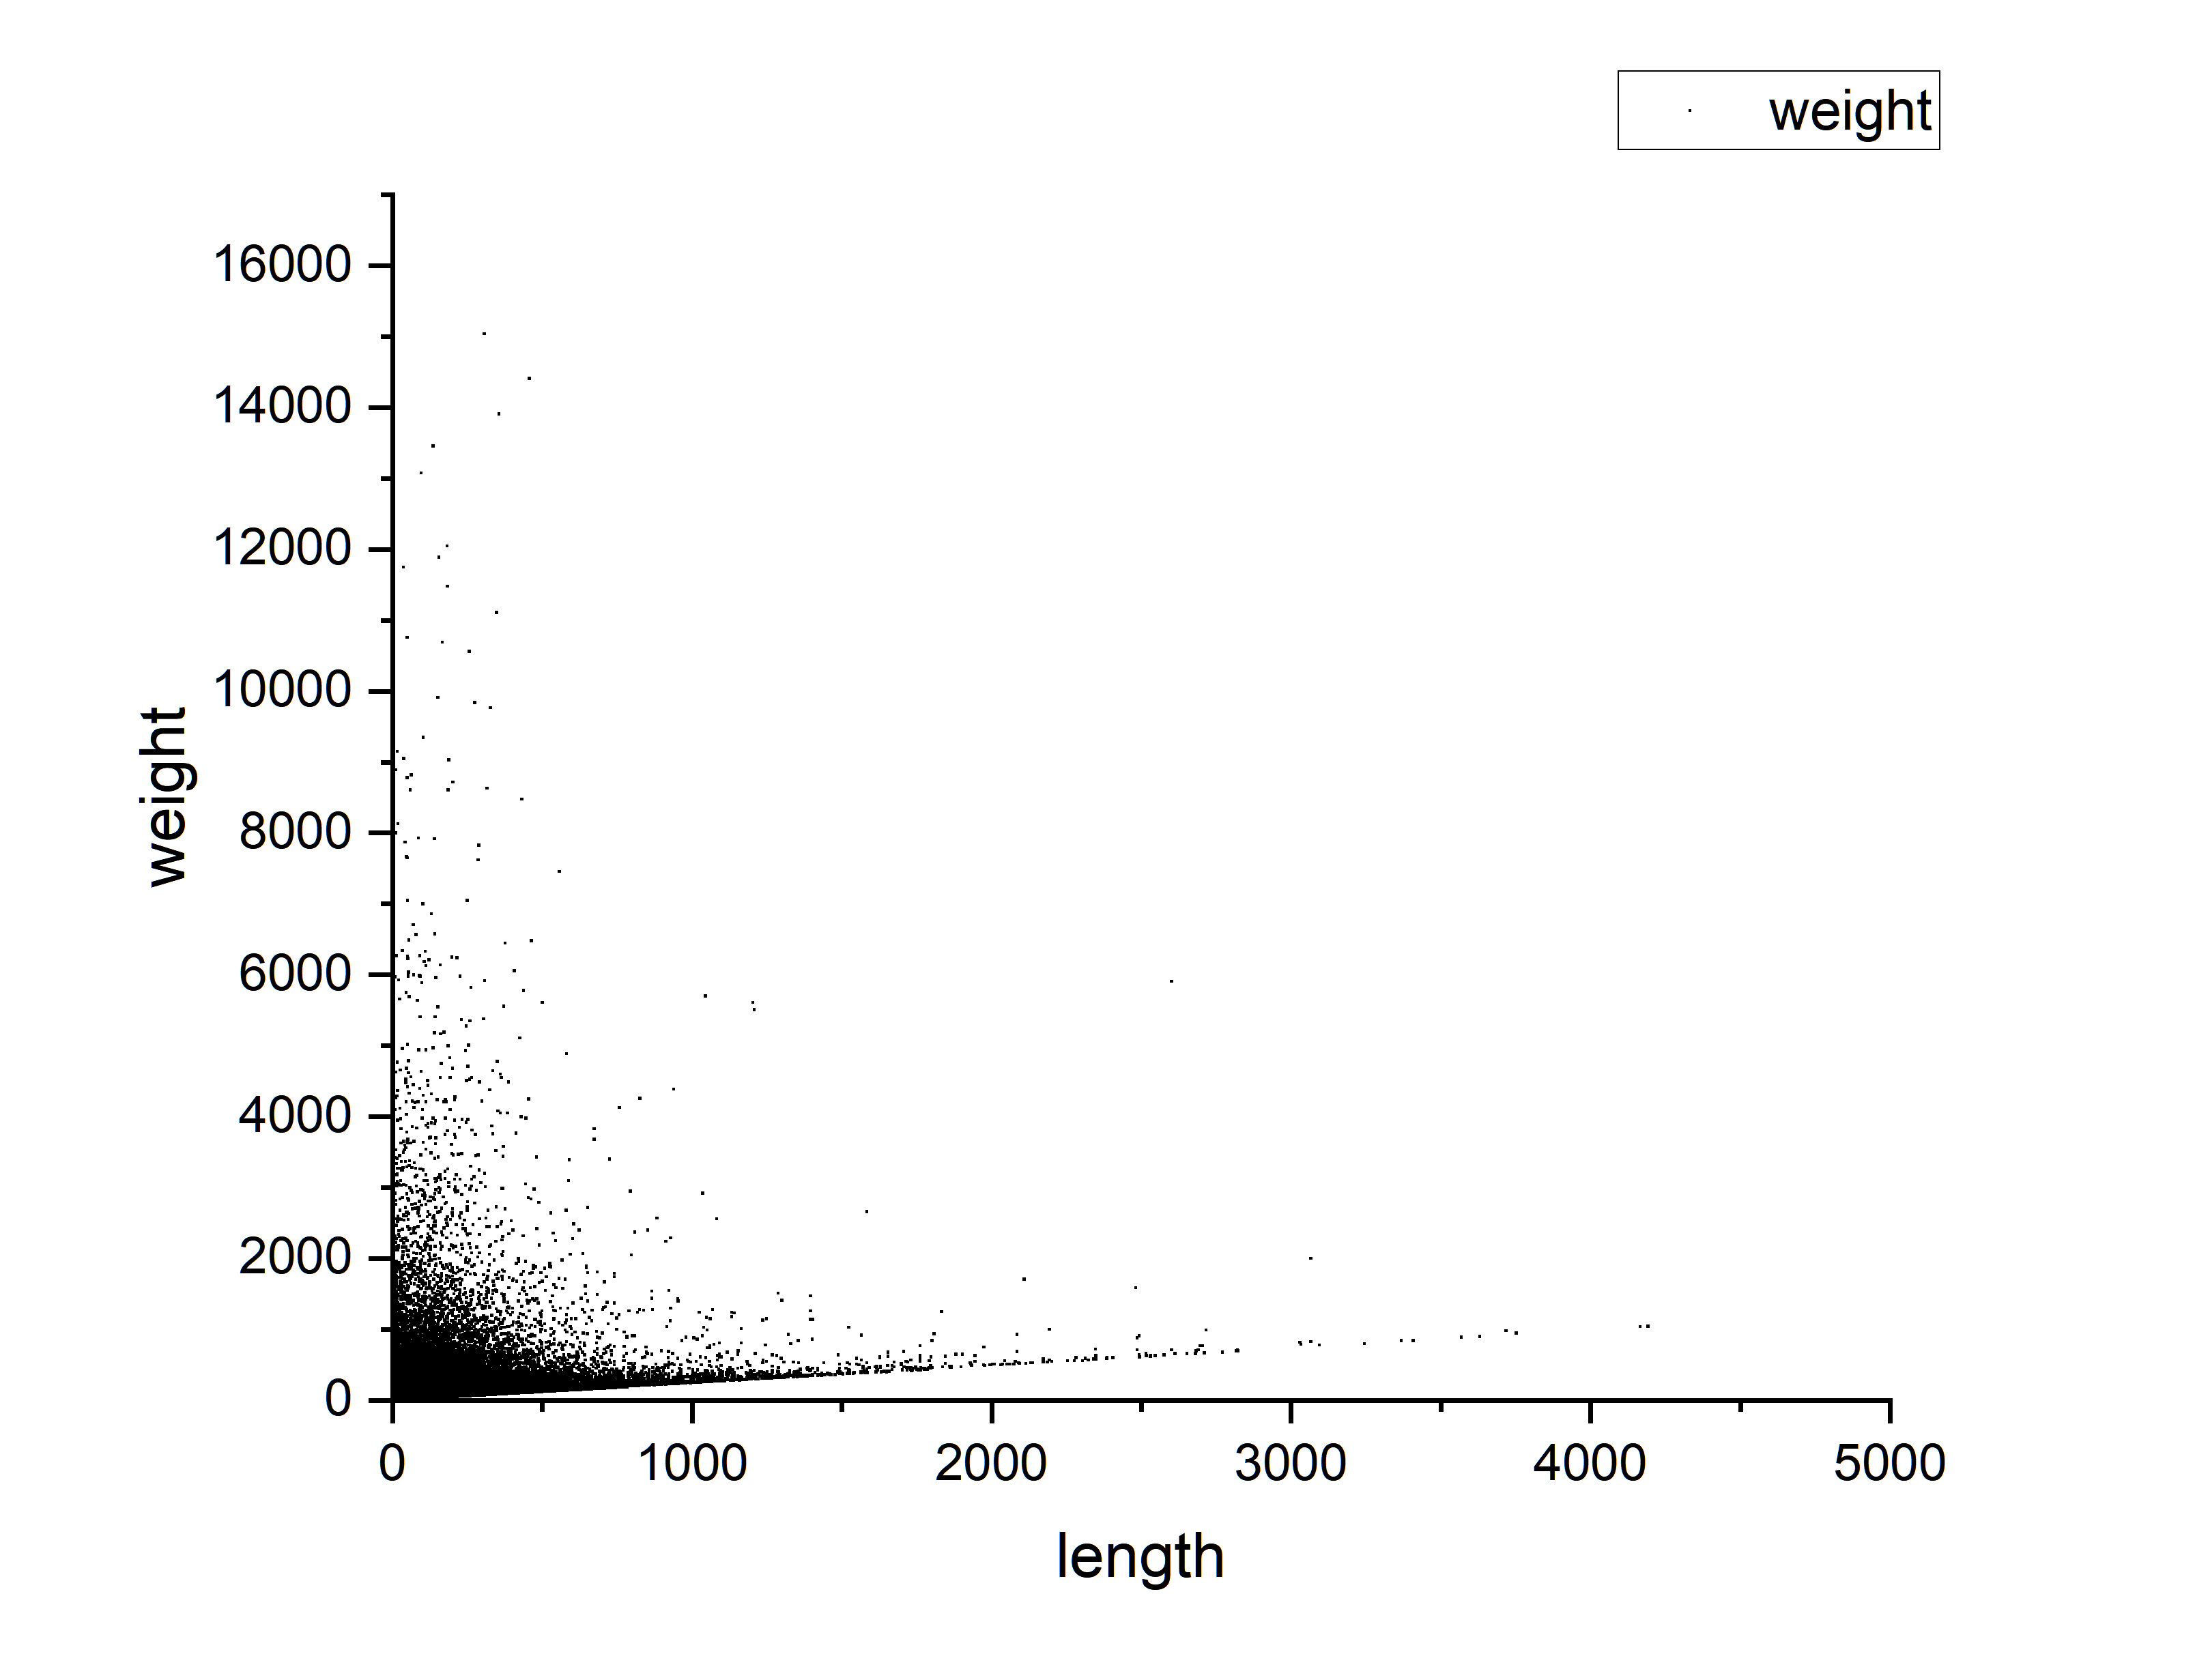
\includegraphics[width=8cm,height=6cm]{weight-length.png}
    \caption{The relationship Between Weight And Length}
\end{figure}
\indent From the Figure 14,  the relationship between edge weights and edge lengths is not always linear. When the length is short, the weight varies significantly, indicating that people are less likely to choose some edges even if they are short in distance. As the edge length gradually increases, the weight generally tends to increase, and the weight becomes more stable with smaller variations. This indicates that most of the time people are unwilling to take detours. However, there are also edges with significantly lower weights when the length is larger. The presence of these edges is usually due to people wanting to avoid specific locations or needing to reach specific attractions.\\
\indent To provide a more detailed explanation of the reasons for these differences, we compared the differences between edge PageRank and edge length, and plotted a scatter plot to illustrate this:
\begin{figure}[H]%插入图片:weight-length
    \centering
    \subfigure{
        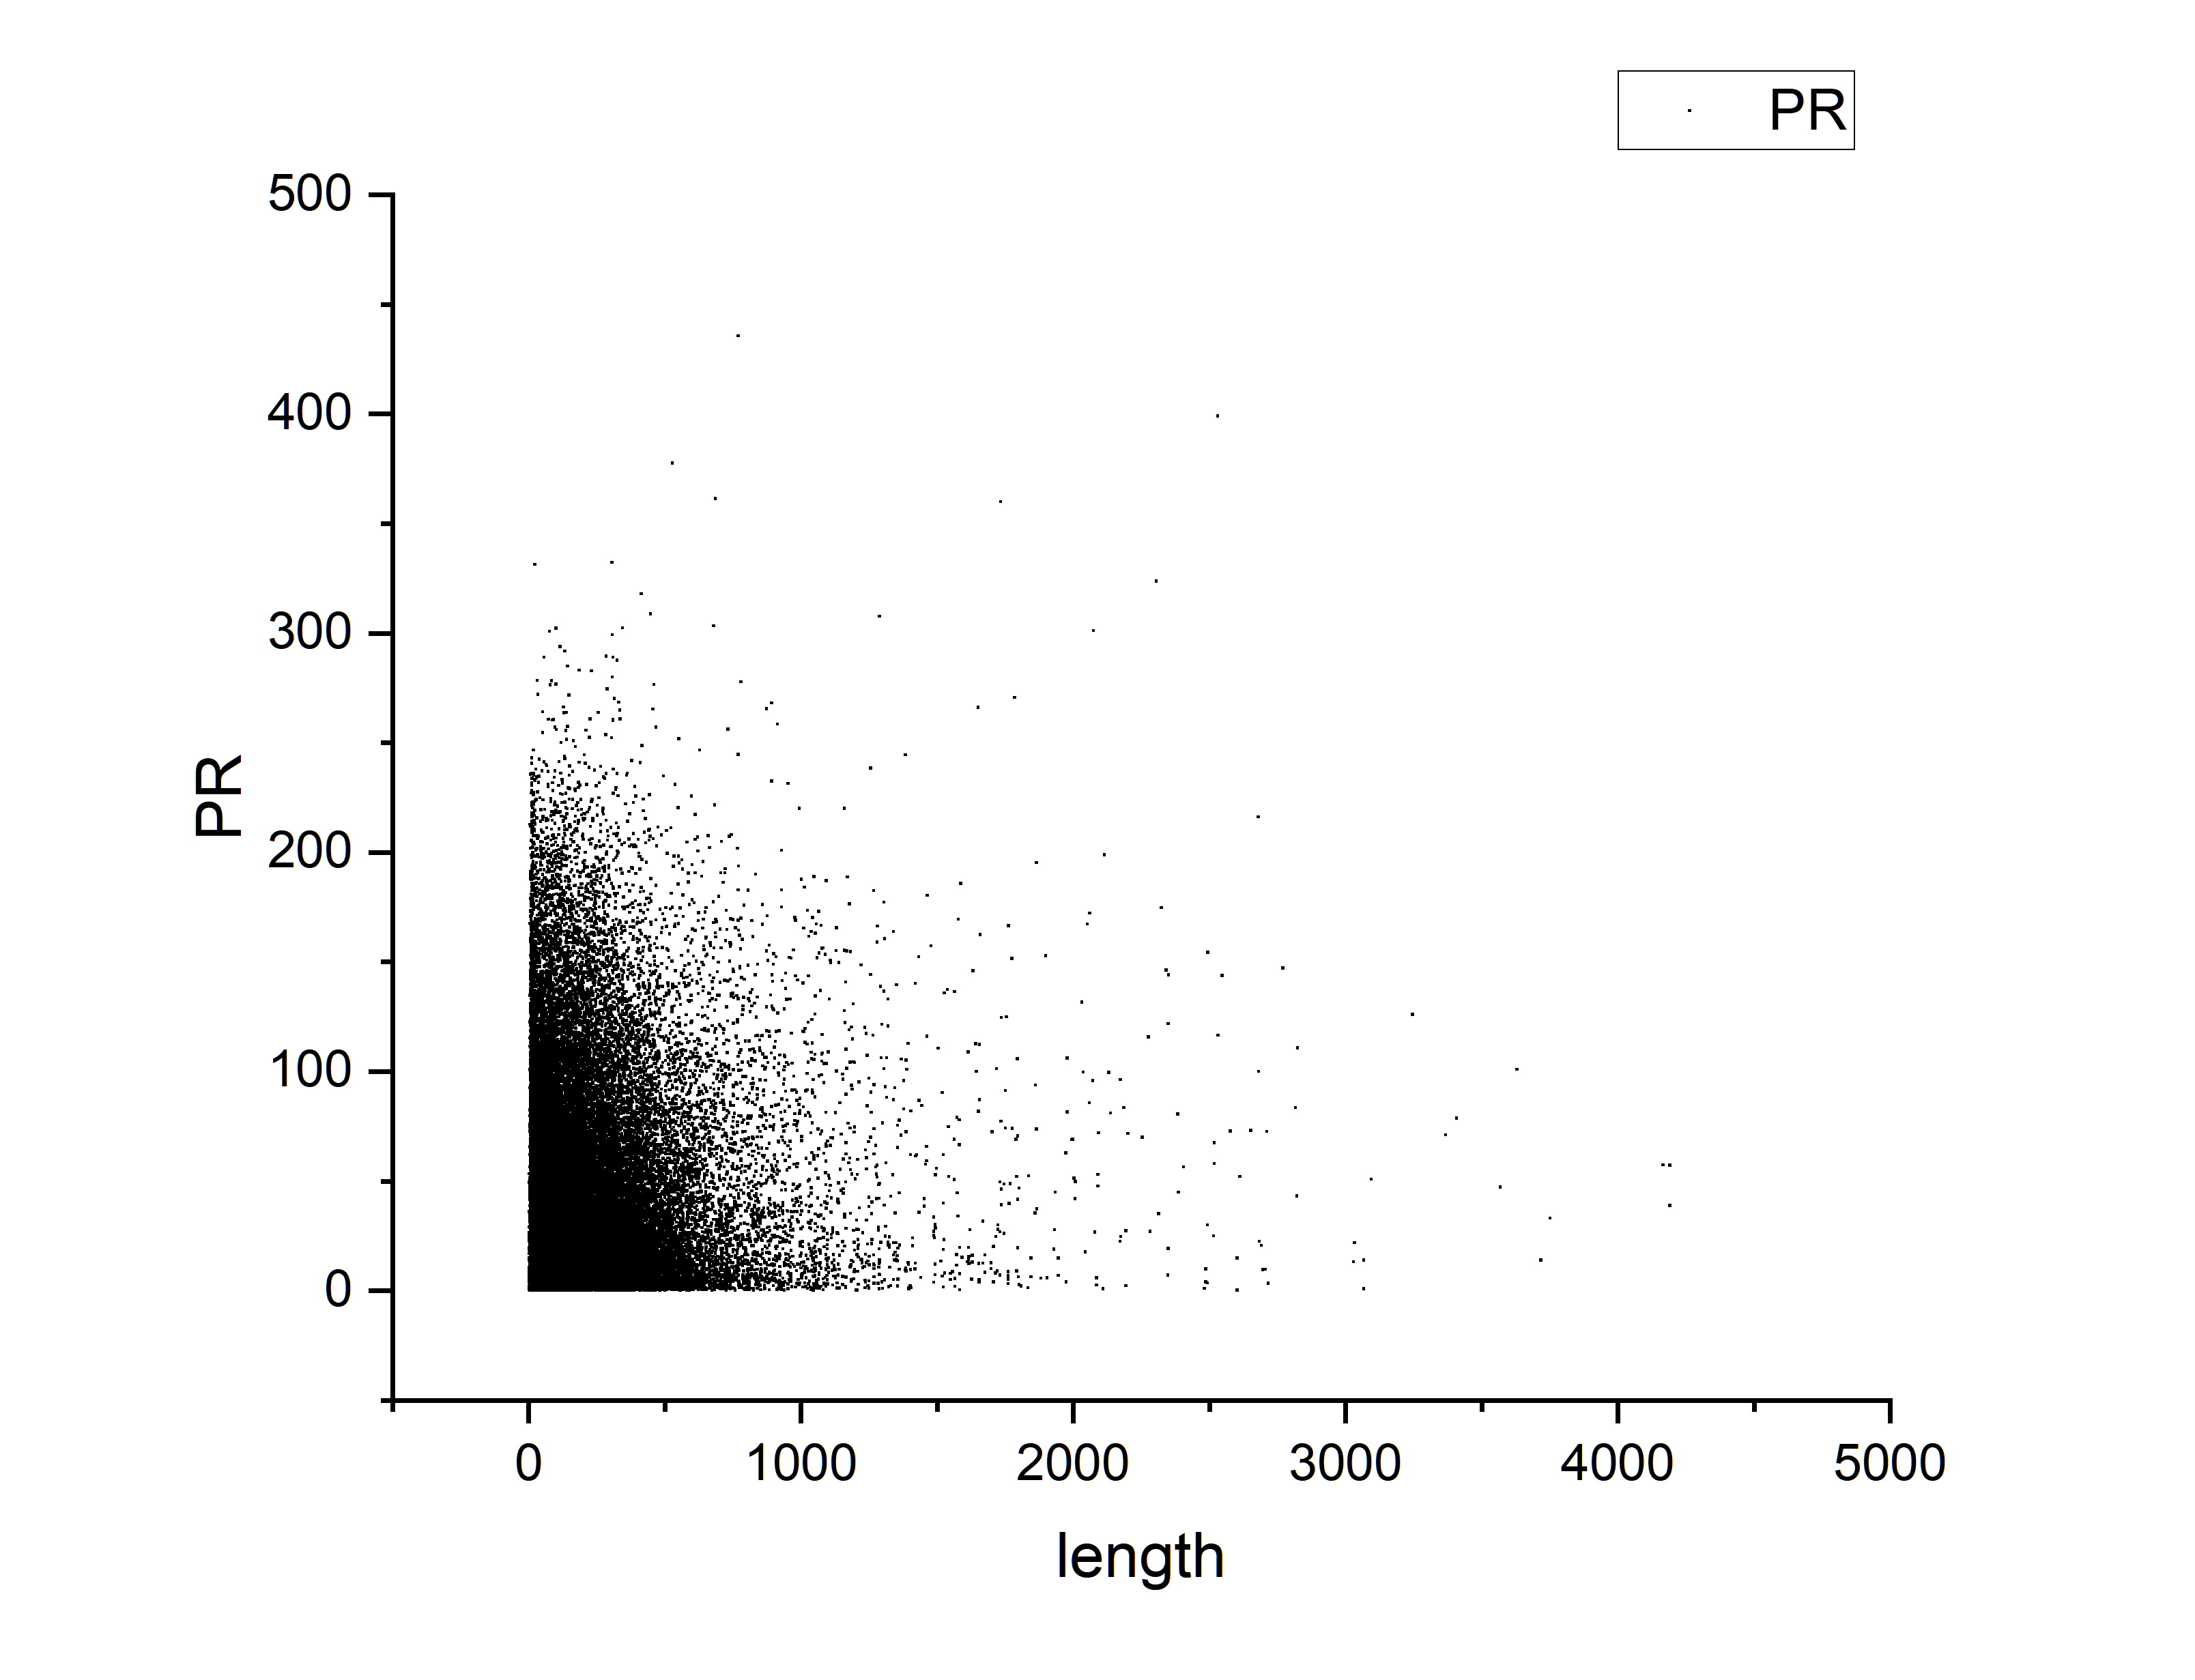
\includegraphics[width=6cm,height=4.5cm]{PR-length.png}}
    \subfigure{
        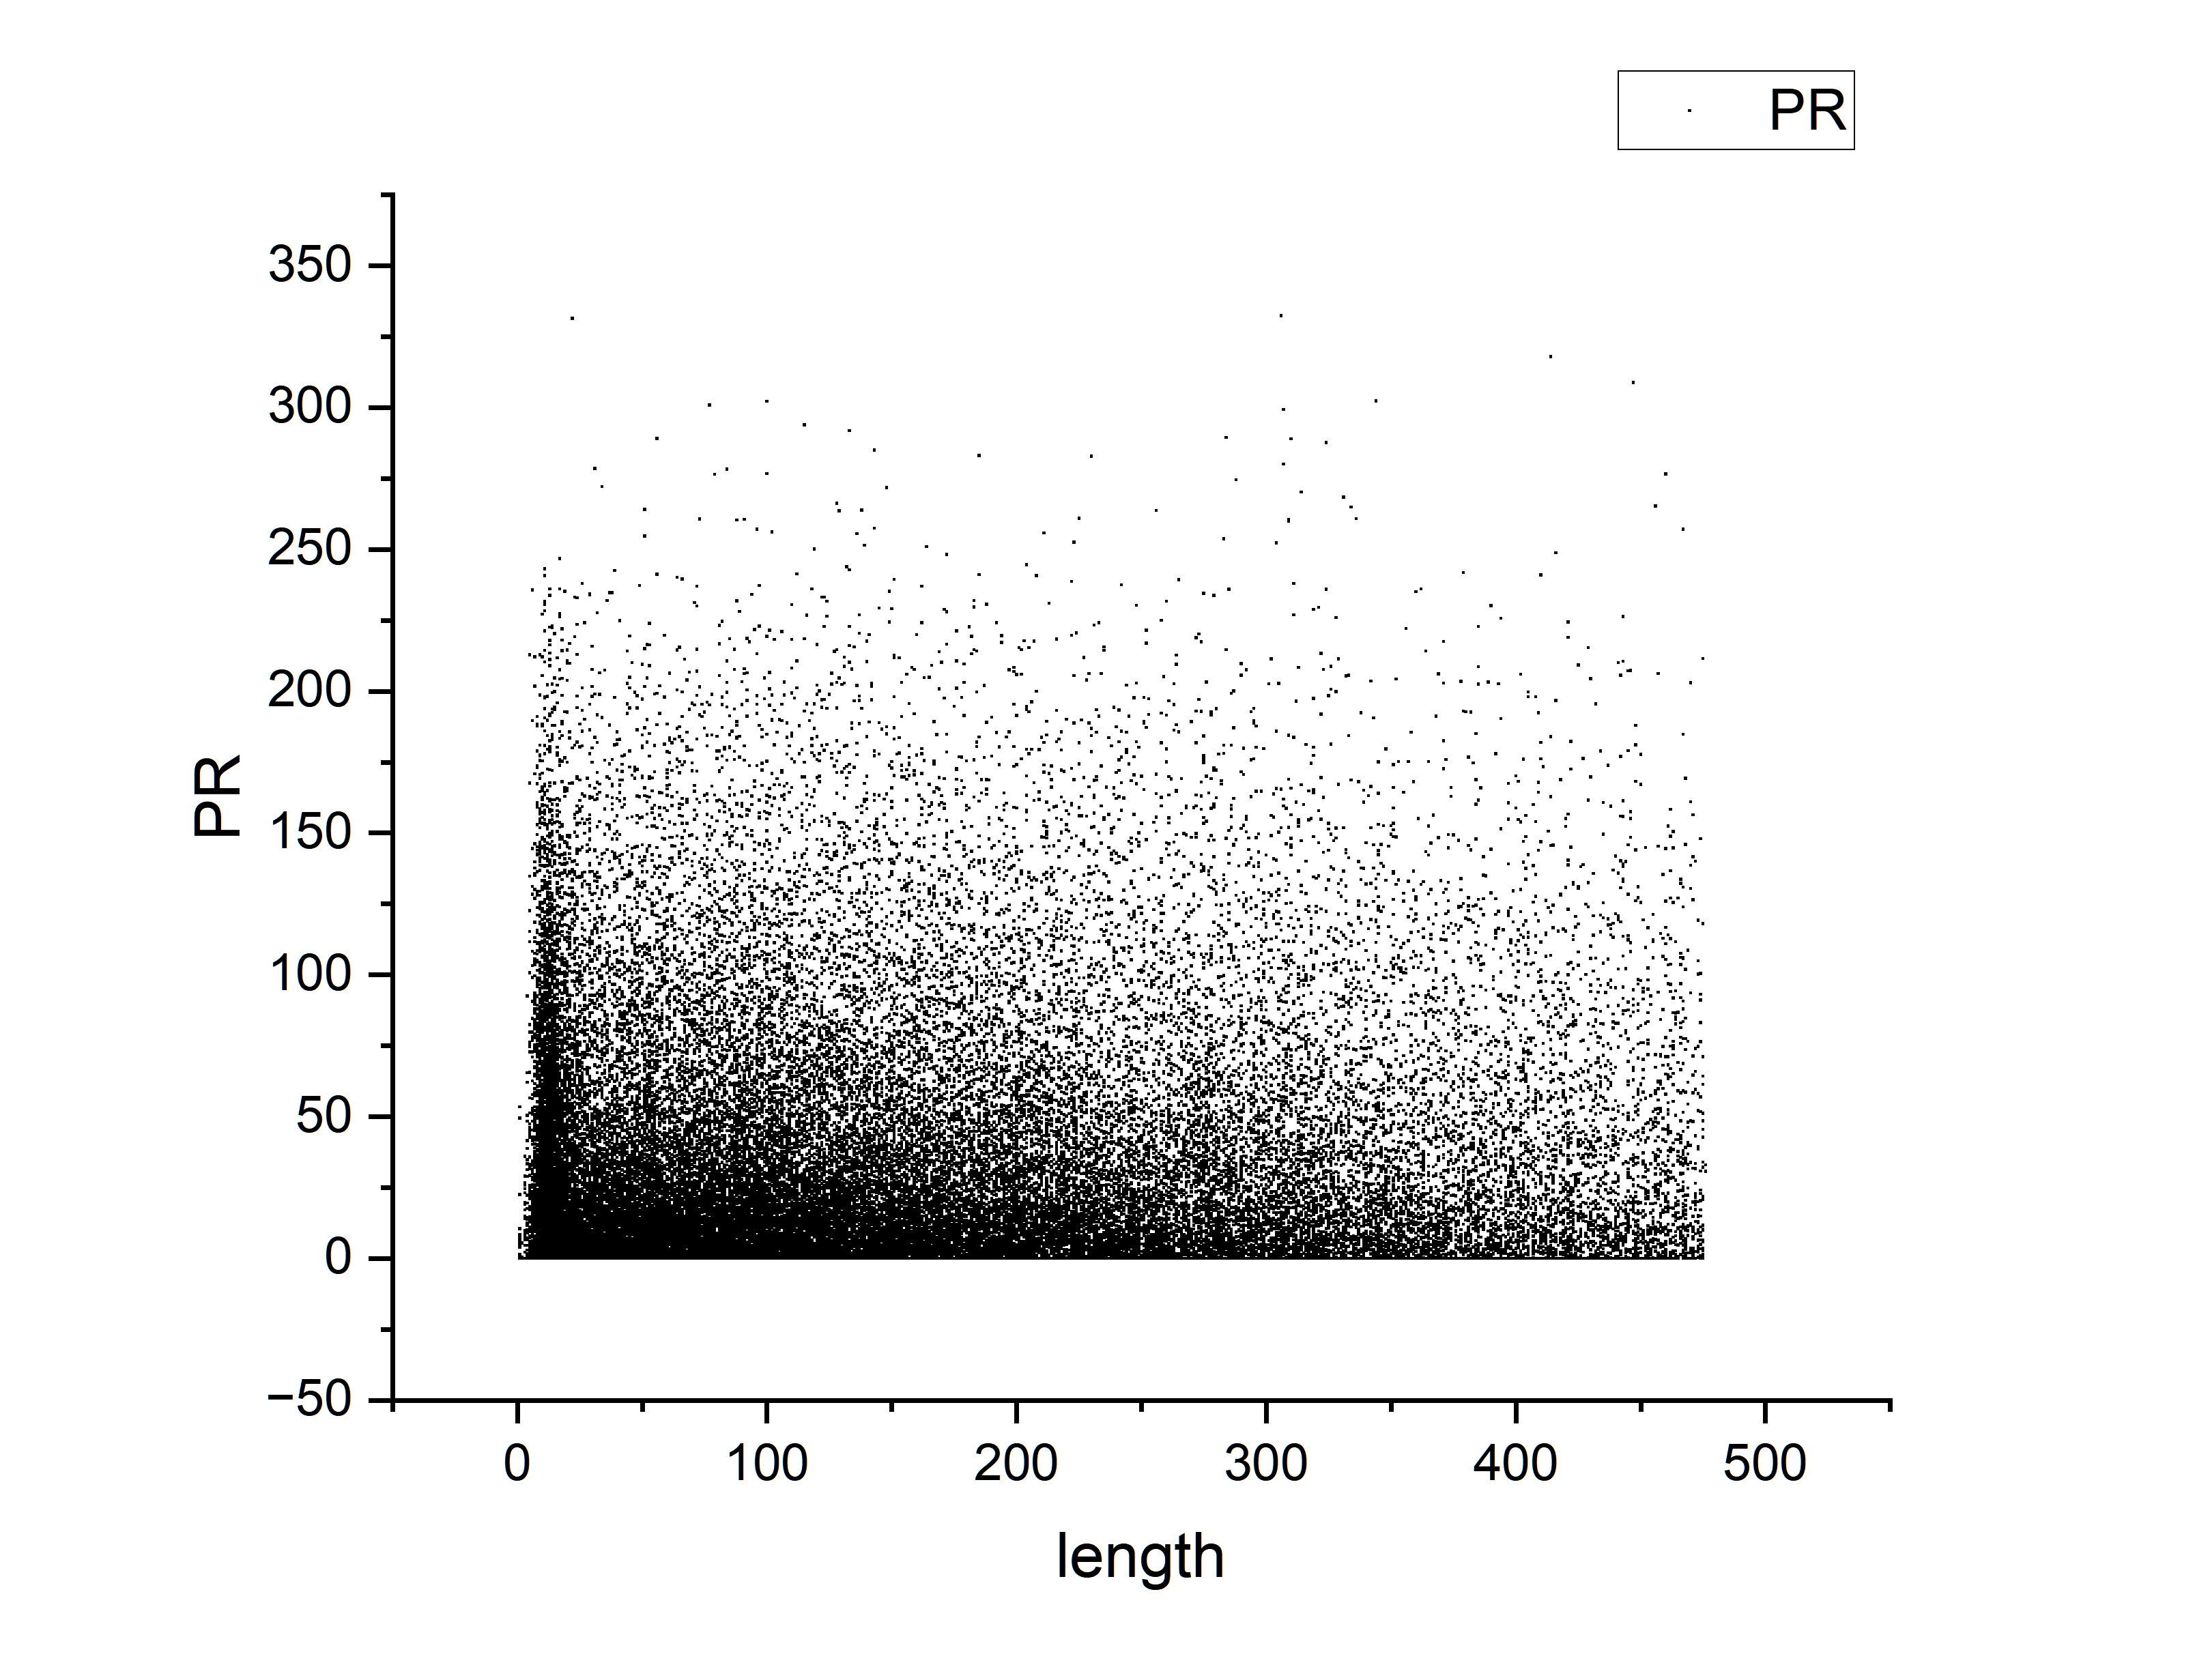
\includegraphics[width=6cm,height=4.5cm]{PR-length 0 to 500.png}}
    \caption{The relationship Between PR And Length}
\end{figure}
\indent The left figure shows the relationship between the PageRank values (PR) of all points and their corresponding lengths (length). The right figure is a zoomed-in view of the left figure, focusing on the part where the length is less than 500. It is evident that when the length is small, there is a larger variation in PR values, whereas as the length increases, the PR values gradually stabilize.\\
\indent By taking into account these two factors, we can effectively determine the weights of the roads. With the consideration of user experience, we have identified the optimal path for selection.






\section{Testing}
\indent\indent We have a model based on the simulated annealing algorithm, which is influenced by various parameters such as the maximum value of parameter variation (strides) and initial and final temperatures. We will conduct stability tests on these two parameters to evaluate the stability of the model.\\
\indent First, we keep the initial and final temperatures and parameter values unchanged in the algorithm. We adjust the strides to be 0.3 and 0.6, respectively, and run the program. The final results are as follows:
\begin{figure}[H]
    \centering
    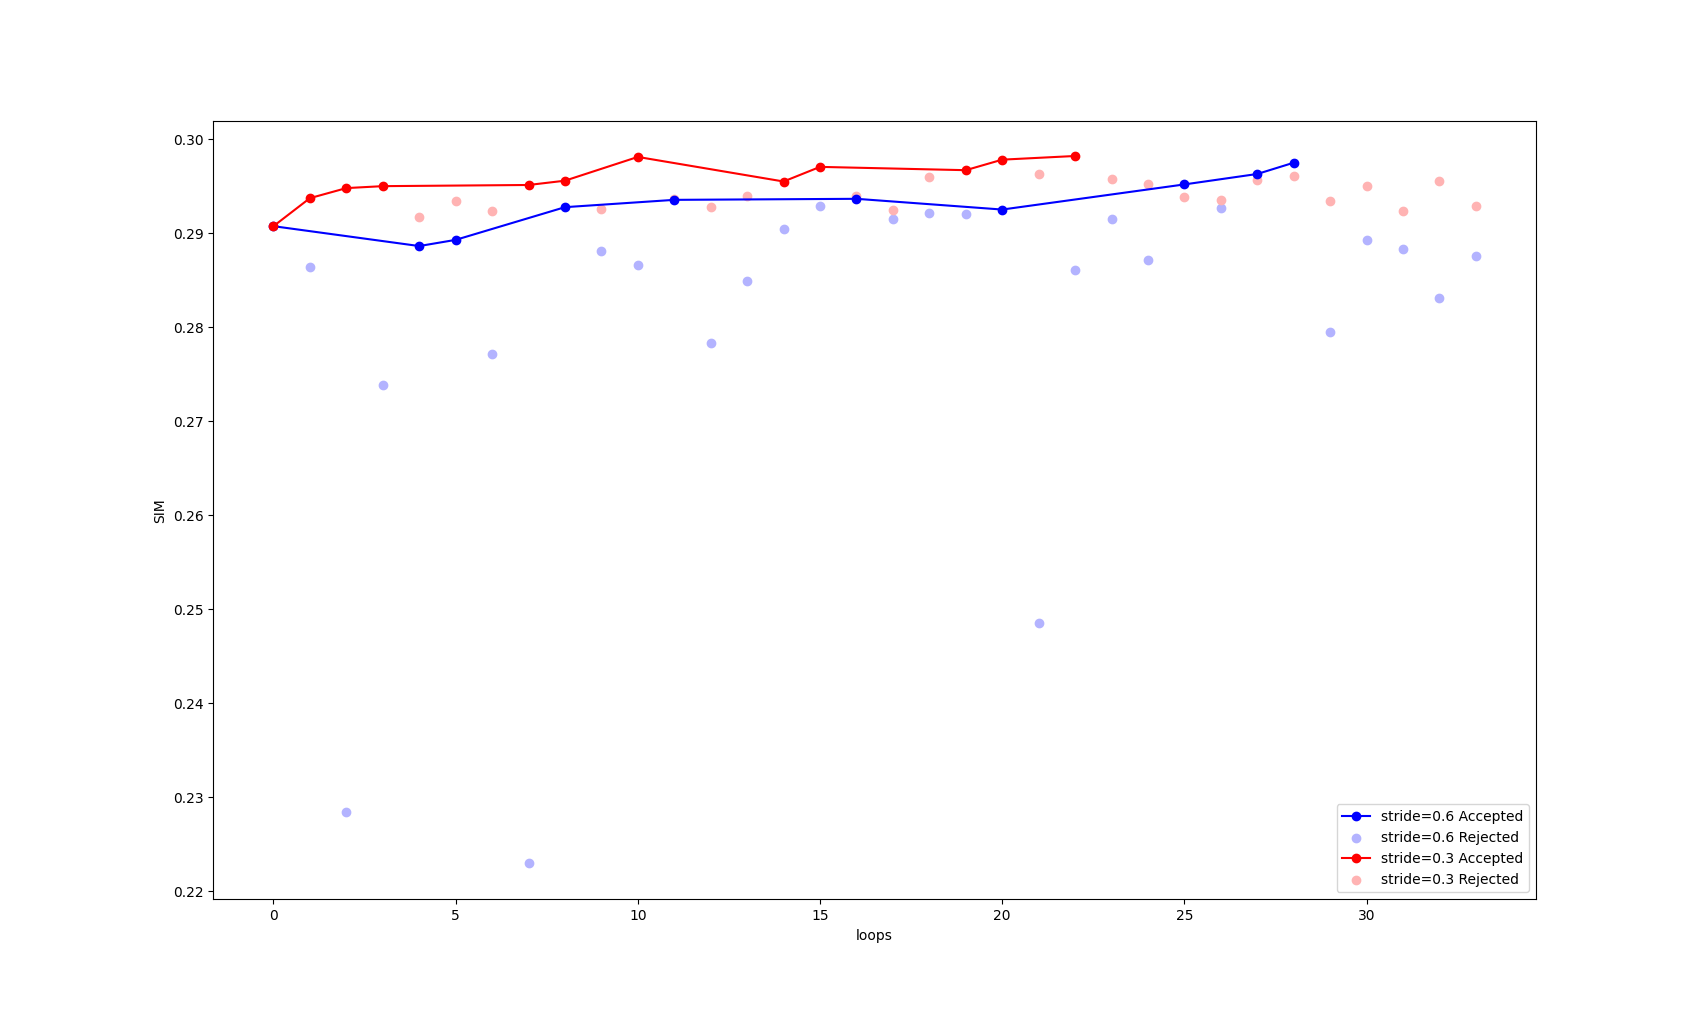
\includegraphics[width=10cm,height=7.5cm]{不同步长.png}
    \caption{SIM with Different Strides}
\end{figure}
\indent We can see that the group with a smaller step size reached the optimum value first and then remained relatively stable. On the other hand, the group with a larger step size took longer to reach the optimum value. The maximum SIM values obtained from the two groups with different step sizes are close, indicating that the model is not sensitive to this parameter.\\
\indent Next, we kept the initial values and strides of all parameters unchanged and only adjusted the initial and final temperatures of the algorithm to be (50,1) and (25,0.5) with a purpose of controlling the rounds. The results are as follows:
\begin{figure}[H]
    \centering
    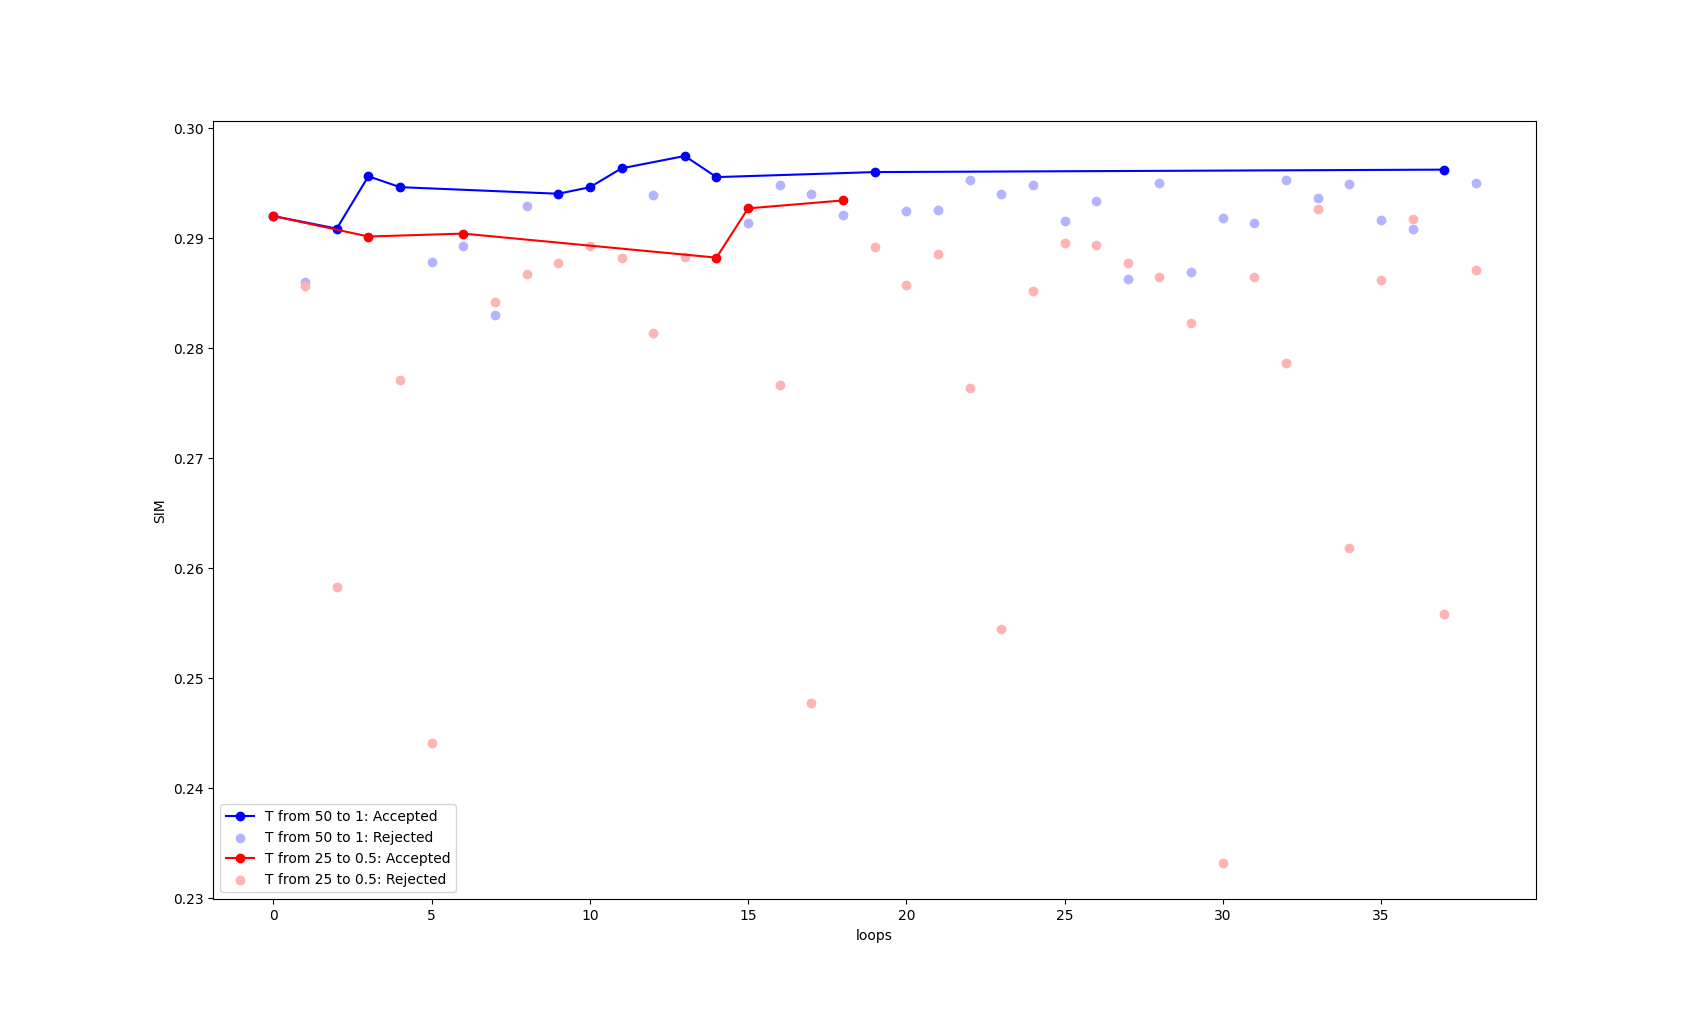
\includegraphics[width=8cm,height=6cm]{T.png}
    \caption{SIM with Different Initial and Final Temperatures}
\end{figure}
\indent We found that the group with a higher initial temperature calculated relatively higher results, while the group with a lower temperature had a lower probability of accepting smaller values, making it easier to reject smaller values and resulting in relatively lower results. However, there was no significant difference between the two groups, indicating a stable performance.\\
\indent To better showcase the tests we conducted, we have created the following table for comparison:
\begin{table}[H]%绘制结果权值表
    \begin{center}
        \caption{Robustness Test}{\vspace{0.5cm}}
        \begin{tabular}{cc}
        \hline
        \text{Trial}&\text{$SIM_{max}$}\\
        \hline
        \text{$T_0$=50  $T_{end}$=1 strides=0.3}&0.296183\\
        \hline
        \text{\quad $T_0$=25 $T_{end}$=0.5 strides=0.3}&0.293384\\       
        \hline
        \text{$T_0$=30  $T_{end}$=1 strides=0.6}&0.297507\\  
        \hline
        \text{$T_0$=30  $T_{end}$=1 strides=0.3}&0.298223\\       
        \hline
        \end{tabular}
    \end{center}
    \end{table}
\indent Considering the two indicators above, we believe that \textbf{our model exhibits strong stability and is not sensitive to changes in parameters}.


\section{Strengths and Weaknesses}
\subsection{Strengths}
\subsection{Weaknesses}

\newpage
\section{References}
\begin{thebibliography}{99}
	\bibitem{1}\url{http://www.google.com/}
	\bibitem{2}Ronneberger O, Fischer P, Brox T. U-net: Convolutional networks for biomedical image segmentation[C]//International Conference on Medical image computing and computer-assisted intervention. Springer, Cham, 2015: 234-241.
\end{thebibliography}
\appendix{\textbf{Appendix}\Huge}
\begin{verbatim}
    inline void Dijkstra(int s, int* d, int numv, vector<Edge>* adj, unordered_map<pair<int, int>, Edge, pair_hash>& map)
    {
        priority_queue<pair<int, int>, vector<pair<int, int>>, greater<pair<int, int>>> q;
        bool visited[maxV];
        for (int i = 0; i < numv; i++)
            d[i] = maxD;
        memset(visited, 0, sizeof(visited));
        d[s] = 0;
        int mind = maxD;
        int now = 0;
        q.push({ 0, s });
        while (true) {
            mind = maxD;
            if (q.empty())
                return;
            auto x = q.top();
            q.pop();
            int now = x.second, mind = x.first;
            if (visited[now])
                continue;
            visited[now] = 1;
            for (int i = 0; i < adj[now].size(); i++) {
                int to = adj[now][i].end;
                if (d[now] + map[{now, to}].weight < d[to])
                {
                    d[to] = d[now] + map[{now, to}].weight;
                    q.push({ d[to], to });
                }
            }
        }
    }
\end{verbatim}
\begin{verbatim}
    static double SIM(unordered_map<pair<int, int>, Edge, pair_hash>& map, vector<Edge>* edges) {
	ifstream file("path.txt");//data-processed
	string line;
	int simcnt = 0, cnt = 0, start0 = -1;
	int d[maxV];
	while (getline(file, line)) {
		istringstream ss(line);

		int pathlength = 0;
		int start, end;
		ss >> start;
		if (start0 != start) {
			dijkstra(start, d, numv, edges, map);
			start0 = start;
		}
		while (ss >> end) {
			pathlength += map[{start, end}].weight;
			start = end;
		}
		if (pathlength == d[end]) {
			simcnt++;
		}
		cnt++;
	}

	file.close();
	return 1.0 * simcnt / cnt;
}

\end{verbatim}

\begin{verbatim}
    static void Page_Rank(vector<Edge>* adj, vector<Edge>* antiadj, int numv, double* b, double a) {
	vector <Edge>new_Adj[maxV];
	vector <Edge>new_Antiadj[maxV];
	for (int i = 0; i < numv; i++) {
		double pr = 0;
		for (int k = 0; k < antiadj[i].size(); k++)
			pr += antiadj[i][k].weight;
		pr *= a;
		pr += b[i];
		pr /= adj[i].size();
		for (int j = 0; j < adj[i].size(); j++)
		{
			add_Edge(i, adj[i][j].end, pr, new_Adj);
			add_Edge(adj[i][j].end, i, pr, new_Antiadj);
		}
	}
	for (int i = 0; i < numv; i++)
	{
		for (int j = 0; j < adj[i].size(); j++)
			adj[i][j] = new_Adj[i][j];
		for (int j = 0; j < antiadj[i].size(); j++)
			antiadj[i][j] = new_Antiadj[i][j];
	}
}
\end{verbatim}

\begin{verbatim}
    struct pa {
	double a, b, c;
};
static pa SA(pa now, unordered_map<pair<int, int>, Edge, pair_hash>& pr, unordered_map<pair<int, int>, Edge, pair_hash>& length, vector<Edge>* edges, vector<Point> v) {
	unordered_map<pair<int, int>, Edge, pair_hash> weight;
	cal_weight(now, weight, pr, length, v);
	double sim1, sim2, dsim;
	sim1 = SIM(weight, edges);
	double T = 25, T_end = 0.5;
	while (T > T_end) {
		pa par = update(now);
		cal_weight(par, weight, pr, length, v);
		sim2 = SIM(weight, edges);

		dsim = (sim2 - sim1) * 10000;
			double r;
			r = (double)rand() / RAND_MAX;
			if (r < exp(dsim / T)) {
				now = par;
				sim1 = sim2;
			}
		}
		else {
			now = par;
			sim1 = sim2;
		}
		T *= 0.9;
	}
	myfile.close();
	return now;
}
\end{verbatim}
   





%%%%%%%%%%%%%%%%%%%%%%%%%%%%%%
\end{document}
\end